\documentclass[11pt,a4paper,twoside,
openright]{book}
\usepackage[italian]{babel}
\usepackage{fullpage}
\usepackage{amsmath}
\usepackage{mathtools}
\usepackage{amsthm}
\usepackage{amssymb}
\usepackage{amsfonts}
\usepackage{tikz-cd}
\usepackage{cite}
\usepackage{chngcntr}
\usepackage[utf8x]{inputenc}
\usepackage{enumerate}
\usepackage{makeidx}
\usepackage{pgf}
\usepackage{tikz}
\usepackage{changepage}
\usepackage{booktabs}
\usepackage{url}
\usepackage{dcolumn}

\usetikzlibrary{decorations.pathreplacing}
\usetikzlibrary{fadings}
\usetikzlibrary{positioning,calc}
\usetikzlibrary{arrows,shapes,snakes,automata,backgrounds,petri}
\tikzset{basic/.style={draw,fill=blue!50!green!20,
                       text badly centered,minimum width=3em}}
\tikzset{input/.style={basic,circle}}
\tikzset{weights/.style={basic,rectangle,minimum width=2em}}
\tikzset{functions/.style={basic,circle,fill=blue!50!green!20}}
\newcommand{\addsymbol}{\draw[thick] (0.5em,0.5em) -- (0,0.5em) -- 
                        (0,-0.5em) --  (-0.5em,-0.5em)
                        (0em,0.75em) -- (0em,-0.75em)
                        (0.75em,0em) -- (-0.75em,0em);}
\DeclarePairedDelimiter{\ceil}{\lceil}{\rceil}
\renewcommand{\contentsname}{Indice}
\newcommand{\matr}[1]{\mathbf{#1}} 

\begin{document}

\begin{titlepage}
	
	\begin{figure}
		\centering
		
\includegraphics[width=424pt]{tesiSCIENZE_TECNOLOGIE.jpg}%A QUESTO LINK TROVATE I MARCHI PER LA TESI AGGIORNATI E DIVISI PER FACOLTà: http://www.unimi.it/ateneo/37094.htm
		\vspace{0.5 cm}
	\end{figure}
	
%DATO CHE NEI MARCHI SONO GIà PRESENTI SIA IL NOME DELL'UNIVERSITà SIA QUELLO DELLA FACOLTà, NON VANNO RISCRITTI. IN OGNI CASO AGGIUNGO IN COMMENTO COME SAREBBERO:	
%\begin{center}
%	{\Huge \textsc{Università degli Studi di Milano} }\\
%\end{center}
%\begin{center}
%{\Huge Facoltà XXXXX}\\
%\end{center}

\begin{center}
{\LARGE Corso di Laurea in Informatica}
\end{center}

\begin{center}
\vspace{3 cm}
{\LARGE \textsc{Compressione di reti neurali \\[5pt] in problemi  di classificazione e regressione} }
\end{center}
\par
  \vspace{3 cm}
  
  \begin{flushleft}
  		 Relatore:\\Prof. Dario MALCHIODI\\
		 
  		 \noindent Correlatore:\\Dr. Marco FRASCA
  \end{flushleft}
  \vspace{1 cm}
  \begin{flushright}
  	Tesi di Laurea di:\\ Giosuè Cataldo Marinò\\ Matricola: 829404
  \end{flushright}
    	  
\vfill
\begin{center}
	{\large Anno Accademico 2018/2019}
\end{center}

\end{titlepage}


\tableofcontents

\chapter*{Introduzione}
Le reti neurali offrono un insieme di strumenti molto potente che permette di risolvere problemi nell'ambito della classificazione, della regressione e del controllo non-lineare. Un semplice esempio è l'analisi di un'immagine riconoscendo il tipo e la posizione degli oggetti nel primo caso e convertendo l'immagine in testo scritto nel secondo.
Oltre ad avere un'elevata velocità di elaborazione, le reti neurali hanno la capacità di imparare la soluzione di un problema a partire da un insieme di sue istanze. In molte applicazioni questo permette di raggirare il bisogno di sviluppare un modello dei processi fisici alla base del problema, che spesso può essere difficile, se non impossibile, da trovare.
L'ispirazione per le reti neurali deriva dagli studi sui meccanismi di elaborazione dell'informazione nel sistema nervoso biologico, in particolare il cervello umano; infatti, gran parte della ricerca sulle reti ha proprio lo scopo di capire più a fondo questi meccanismi.
Dalle loro origini ad oggi, sono stati sviluppati numerosi modelli di reti neurali per risolvere problemi di diversa natura, tuttavia qui sarà presentato il modello conosciuto come multilayer perceptron. Esso fa parte di una classe di modelli di reti
generica conosciuta come reti feedforward, ovvero reti in cui l'informazione si muove in un'unica direzione e in cui non ci sono cicli.
Due dei principali problemi delle reti neurali sono il tempo di addestramento e lo spazio necessario per memorizzare le strutture dati; entrambi questi problemi sono dovuti a numerosi fattori  quali specifiche della macchina, complessità, dimensione degli input e numero di parametri. Per quest'ultimo fattore, la ricerca di metodi di compressione è fondamentale per cercare di ridurre l'impatto degli svantaggi di una rete su un sistema. 
In questo elaborato si analizza l'impatto di due algoritmi di compressione sulla performance di reti neurali, analizzando in particolare la variazione della loro accuratezza per un problema di classificazione e un problema di regressione, considerando diversi dataset.
L'elaborato è strutturato nel modo seguente: nel Capitolo 1 viene fornito un quadro semplificato del funzionamento delle reti neurali biologiche, in modo da trovare una corrispondenza pratica dei concetti riguardanti le reti neurali artificiali; oltre a descrivere la struttura del modello MLP in dettaglio, parleremo di una tecnica usata per addestrarla. Nel Capitolo 2 vengono descritte due tecniche di compressione per le reti neurali, spiegandone il funzionamento, le strutture dati necessarie e il loro tasso di compressione.
Nel Capitolo 3 vengono applicate le tecniche di compressione esplicate nel capitolo precedente mostrando confronti tra diverse reti. Il lavoro è chiuso con alcune considerazioni finali.
\chapter{Reti Neurali}
In questo capitolo descriveremo le reti neurali artificiale, partendo dall'analogia con il sistema nervoso. Successivamente vengono descritti i modelli multilayer-perceptron e un metodo di apprendimento di questo modello.
\section{Reti Neurali Biologiche}
I neuroni sono delle celle elettricamente attive e il sistema nervoso centrale ne contiene circa $10^{11}$. La maggior parte di essi ha la forma indicata in Figura~\ref{fig:neurbio}. I dendriti rappresentano gli ingressi del neurone mentre l’assone ne rappresenta l’uscita. La comunicazione tra i neuroni avviene alle giunzioni, chiamate sinapsi. Ogni neurone è tipicamente connesso ad un migliaio di altri neuroni e, di conseguenza, il numero di sinapsi nel cervello supera $10^{14}$.
\begin{figure}[h!]
\begin{center}
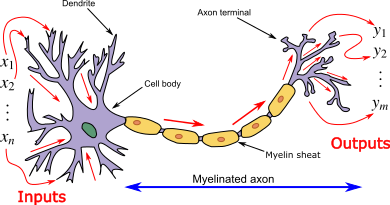
\includegraphics[width=280pt]{BioNeuron.png}
\caption{Neurone Biologico~\cite{pict_neur}}
\end{center}
\label{fig:neurbio}
\end{figure}

Ogni neurone si può trovare principalmente in 2 stati: attivo o a riposo. Quando il neurone si attiva, esso produce un potenziale di azione (impulso elettrico) che viene trasportato lungo l’assone. Una volta che il segnale raggiunge la sinapsi esso provoca il rilascio di sostanze chimiche (neurotrasmettitori) che attraversano la giunzione ed entrano nel corpo di altri neuroni. In base al tipo di sinapsi, che possono essere eccitatori o inibitori, queste sostanze aumentano o diminuiscono rispettivamente le possibilità che il successivo neurone si attivi. Ad ogni sinapsi è associato un peso che ne determina il tipo e l’ampiezza dell’effetto eccitatore o inibitore. Quindi, semplificando, si può dire che ogni neurone effettua una somma pesata degli ingressi provenienti dagli altri neuroni e, se questa somma supera una certa soglia, il neurone si attiva.\\
Ogni neurone, operando ad un ordine temporale del millisecondo, rappresenta un sistema di elaborazione relativamente lento; tuttavia, l’intera rete ha un numero molto elevato di neuroni e sinapsi che possono operare in modo parallelo e simultaneo, rendendo l’effettiva potenza di elaborazione molto elevata. Inoltre, la rete neurale biologica ha un’alta tolleranza ad informazioni poco precise (o sbagliate), ha la facoltà di apprendimento e generalizzazione.

\section{Reti Neurali Artificiali}
\label{section:retiartificiali}
Ci concentreremo su una classe particolare di modelli di reti neurali: le reti a catena aperta. Queste reti possono essere viste come funzioni matematiche non lineari che trasformano un insieme di variabili indipendenti $x = (x_{1}, ... , x_{d})$, chiamate ingressi della rete, in un insieme di variabili dipendenti $y = (y_{1}, ... , y_{c})$, chiamate uscite della rete. La precisa forma di queste funzioni dipende dalla struttura interna della rete e da un insieme di valori $w = (w_{1}, ... , w_{d})$, chiamati pesi. Possiamo quindi scrivere la funzione della rete nella forma $y = y(x; w)$ che denota il fatto che $y$ sia una funzione di $x$ parametrizzata da $w$.

\begin{figure}[h!]
\begin{center}
\tikzset{basic/.style={draw,fill=white,text width=1em,text badly centered}}
\tikzset{input/.style={basic,circle}}
\tikzset{weights/.style={basic,rectangle}}
\tikzset{functions/.style={basic,circle,fill=white}}
\begin{tikzpicture}[scale=1.2]
    \foreach \h [count=\hi ] in {$x_d$,$x_2$,$x_1$,$1$}{%
          \node[input] (f\hi) at (0,\hi*2cm-5 cm) {\h};
        }
    \node[input] (z) at (10,0) {$z$};
    \node[functions] (sum) at (4,0) {$\sum$};
    \foreach \h [count=\hi ] in {$w_d$,$w_2$,$w_1$,$b$}{%
          \path (f\hi) -- node[weights] (w\hi) {\h} (sum);
          \draw[->] (f\hi) -- (w\hi);
          \draw[->] (w\hi) -- (sum);
        }        
    \node[functions] (step) at (7,0) {};
       \begin{scope}[xshift=7cm,scale=.75]
         \addsymbol
       \end{scope}
    \draw[->] (sum) -- (step);
    \draw[->] (step) -- (z);%++(1,0);
    % Labels
    \node[above=.5cm]  at (f4) {Inputs};
    \node[above=.5cm] at (w4) {Weights};
    
\end{tikzpicture}
\end{center}
\caption{Modello di McCulloch-Pitts}
\label{fig:mcpitts}
\end{figure}
\subsection*{Modello di McCulloch-Pitts}

Un semplice modello matematico di un singolo neurone è quello rappresentato in Figura~\ref{fig:mcpitts} ed è stato proposto da McCulloch e Pitts~\cite{McCulloch:1943aa} alle origini delle reti neurali artificiali. Esso può essere visto come una funzione non lineare che trasforma le variabili di ingresso $x_{1}, ..., x_{d}$ nella variabile di uscita $z$. Nell’elaborato ci riferiremo a questo modello come unità di elaborazione, o semplicemente unità.
In questo modello, viene effettuata la somma ponderata degli ingressi, usando come pesi i valori $w_{1}, ..., w_{d}$ (che sono analoghi alle potenze delle sinapsi nella rete biologica), ottenendo così
\begin{equation}
a = \sum\limits_{i=1}^d w_{i}x_{i}+b
\label{som+b}
\end{equation}
dove il parametro $b$ viene chiamato bias (corrisponde alla soglia di attivazione del neurone biologico). Se definiamo un ulteriore ingresso $x_{0}$, impostato costantemente a 1, possiamo scrivere~\eqref{som+b} come
\begin{equation}
a = \sum\limits_{i=0}^d w_{i}x_{i}
\label{som}
\end{equation}
dove $x_{0}$ = 1. Precisiamo che i valori dei pesi possono essere di qualsiasi segno, che dipende dal tipo di sinapsi. L’uscita $z$ (che può essere vista come tasso medio di attivazione del neurone biologico) viene ottenuta applicando ad $a$ una trasformazione non lineare $g$, chiamata funzione di attivazione, ottenendo 
\begin{equation}
z=g(a)=g\left( \sum\limits_{i=0}^d w_{i}x_{i} \right).
\label{act+som}
\end{equation}
Il modello originale di McCulloch-Pitts usava come attivazione la funzione gradino
\begin{equation}
g(a)=
\begin{cases}
1 &\text{ se } a\geq0, \\
-1 &\text{ altrimenti}.
\end{cases}
\label{act+som}
\end{equation}

\section{Addestramento della rete}
\label{addestramento}
Abbiamo detto che una rete neurale può essere rappresentata dal modello matematico $y = y(x; w)$, che è una funzione di $x$ parametrizzata dai pesi $w$. Prima di poter utilizzare questa rete, dobbiamo identificare il modello, ovvero dobbiamo determinare tutti i parametri $w$. Il processo di determinazione di questi parametri è chiamato addestramento e può essere un’azione molto intensa dal punto di vista computazionale. Tuttavia, una volta che sono stati definiti i pesi, nuovi ingressi possono essere elaborati molto rapidamente.
Per addestrare una rete abbiamo bisogno di un insieme di esempi, chiamato insieme di addestramento (\textit{training set}), i cui elementi sono coppie $(x^{q}, t^{q})$, $q = 1, ..., n$, dove $t^{q}$ rappresenta il valore di uscita desiderato, chiamato target, in corrispondenza dell'ingresso $x^{q}$. 
L’addestramento consiste nella ricerca dei valori per i parametri $w$ che minimizzano un’opportuna funzione di errore. Ci sono diverse forme di questa funzione, la più usata risulta essere la somma dei quadrati residui. I residui sono definiti come
\begin{equation}
r_{qk} = y_{k}\left(x^{q}; w\right) - t^{q}_{k}
\label{res}
\end{equation}
dove $k$ rapppresenta l'indice dei neuroni di output.
La funzione di errore $E$ risulta allora essere
\begin{equation}
E = \sum\limits_{q=1}^n \sum\limits_{k=1}^c r_{qk}^{2}. 
\label{quadres}
\end{equation}
\`E facile osservare che $E$ dipende da $x^{q}$ e da $t^{q}$ che sono valori noti e da $w$ che è incognito, quindi $E$ è in realtà una funzione dei soli pesi $w$.

\section{Funzioni di attivazione}
Come già introdotto nel Paragrafo~\ref{section:retiartificiali}, le funzioni di attivazione determinano l'output di ciascun neurone della rete neurale.
Le funzioni utilizzate principalmente negli esperimenti di questo elaborato sono tre: \textit{sigmoid}, \textit{ReLU} (\textit{Rectified Linear Units}) e \textit{LeakyReLU} descritte in (\ref{sigmoid} -\ref{lrelu}).
Di solito sono funzioni non-lineari e la loro derivata è calcolabile in modo analitico per velocizzare la computazione.

\begin{equation}
\mathrm{sigmoid}(a) = \frac{1}{1+e^{-a}}, \qquad
\mathrm{sigmoid}'(a) = \mathrm{sigmoid}(a)(1-\mathrm{sigmoid}(a)).
\label{sigmoid}
\end{equation}

\begin{equation}
\mathrm{ReLU}(a) = \max(0,a), \qquad
ReLU'(a) = \begin{cases}
1 &\text{ se } a\geq0, \\
0 &\text{ altrimenti}.
\end{cases}
\label{relu}
\end{equation}

\begin{equation}
\mathrm{LeakyReLU}(a) = \begin{cases}
a &\text{ se } a\geq0, \\
- \alpha a &\text{ altrimenti}.
\end{cases} \qquad
\mathrm{LeakyReLU}'(a) = \begin{cases}
1 &\text{ se } a\geq0, \\
-\alpha &\text{ altrimenti}.
\end{cases}
\label{lrelu}
\end{equation}
dove $\alpha$ è un parametro numerico.

La scelta della funzione è guidata dal tipo di problema che si vuole affrontare, per esempio se vogliamo un output compreso tra 0 e 1 sarà più adeguato utilizzare una funzione \textit{sigmoid} rispetto ad una \textit{ReLU}.



\section{MultiLayer Perceptron}
In questo paragrafo parleremo in dettaglio del modello mulilayer perceptron introducendo il concetto di multistrato e descriveremo il metodo di addestramento utilizzato principalmente nel Capitolo~\ref{esperimenti}. Nell’elaborato ci riferiremo a questo modello come MLP.
\subsection{Architettura del modello MLP}
\label{archmlp}
\paragraph{Modello a uno strato}
\def\layersep{2.5cm}

\begin{figure}
\begin{center}
\begin{tikzpicture}[shorten >=1pt,->,draw=black!50, node distance=\layersep]
    \tikzstyle{every pin edge}=[<-,shorten <=1pt]
    \tikzstyle{neuron}=[basic,circle,fill=black!25,minimum size=17pt,inner sep=0pt]
    \tikzstyle{input neuron}=[neuron, fill=white];
    \tikzstyle{output neuron}=[neuron, fill=white];
    \tikzstyle{hidden neuron}=[neuron, fill=white];
    \tikzstyle{annot} = [text width=4em, text centered]

    % Draw the input layer nodes
    \foreach \name / \y in {0,...,3}
    % This is the same as writing \foreach \name / \y in {1/1,2/2,3/3,4/4}
        \node[input neuron] (I-\name) at (0,-\y-1) {$x_\y$};
	\node[input neuron] (I-d) at (0,-4-1) {$x_d$};
    \node (dot) at (0,-4.4) {$\vdots$};
    %\node[annot,pin={[pin edge={->}]right:bias}, left of=I-0] (O) {};
	\node[annot,pin={[pin edge={->}]below:},above of=I-0, node distance=1.5cm] {$bias$};
    % Draw the output layer node
    \node[output neuron, right of=I-1] (O) {$z_1$};
    \node[right of=I-2] (dot) {$\vdots$};
    \node[output neuron, right of=I-3] (O2) {$z_m$};
	%\node[below of=I-1] (dots) {$\vdots$} -- (dots) node[left of=dots] (ldots) {$\vdots$};

    % Connect every node in the input layer with every node in the
    % hidden layer.
    \foreach \source in {0,...,3}
    	\path (I-\source) edge (O);
    \foreach \source in {0,...,3}
    	\path (I-\source) edge (O2);
    \path (I-d) edge (O);
    \path (I-d) edge (O2);

    % Annotate the layers
    
    %\node[annot, node distance=1cm] (input) {Input layer};
    \node[annot, below of=I-d, node distance=2cm] (input) {Input layer};
    \node[annot, right of=input] {Output layer};
\end{tikzpicture}
\end{center}
\caption{MLP a uno strato}
\label{fig:MLP1}
\end{figure}
Nel paragrafo precedente abbiamo trattato la singola unità di elaborazione descritta in~\eqref{act+som}. Se consideriamo ora un insieme di $m$ unità, con ingressi comuni, otteniamo una rete neurale a singolo strato come in Figura~\ref{fig:MLP1}. Le uscite di questa rete sono date da
\begin{equation}
z_j = g\left(\sum\limits_{i=0}^d w_{ij}x_i\right), \quad
j=1,...,m
\label{rete1}
\end{equation}
dove $w_{ij}$ rappresenta il peso che connette l'ingresso $i$ con l'uscita $j$; $g$ è la funzione di attivazione e $x_0=1$ per incorporare il bias, come precedentemente spiegato.

\paragraph{Modello a due strati}
\begin{figure}
\begin{center}
\def\layersep{1.5cm}

\begin{tikzpicture}[
   shorten >=1pt,->,
   draw=black!50,
    node distance=\layersep,
    every pin edge/.style={<-,shorten <=1pt},
    neuron/.style={circle,basic,fill=black!25,minimum size=17pt,inner sep=0pt},
    input neuron/.style={neuron, fill=white},
    output neuron/.style={neuron, fill=white},
    hidden neuron/.style={neuron, fill=white},
    annot/.style={text width=4em, text centered}
]
	
	\foreach \name / \y in {0,...,2}
    % This is the same as writing \foreach \name / \y in {1/1,2/2,3/3,4/4}
        \node[input neuron] (I-\name) at (0,-\y-1) {$x_\y$};
	\node[input neuron] (I-d) at (0,-3-1) {$x_d$};
    \node (dot) at (0,-3.4) {$\vdots$};

    % Draw the input layer nodes
    %\foreach \name / \y in {1,...,4}
    % This is the same as writing \foreach \name / \y in {1/1,2/2,3/3,4/4}
    %    \node[input neuron, pin=left:Input \#\y] (I-\name) at (0,-\y) {};

    % set number of hidden layers
    \newcommand\Nhidden{1}

    % Draw the hidden layer nodes
    
	\foreach \y in {0,...,4}
    % This is the same as writing \foreach \name / \y in {1/1,2/2,3/3,4/4}
        \node[input neuron] (H-\y) at (\layersep,-\y) {$z_\y$};
	\node[input neuron] (H-m) at (\layersep,-5) {$z_m$};    
    \node (dot) at (\layersep,-4.4) {$\vdots$};

    %\foreach \N in {1,...,\Nhidden} {
    %   \foreach \y in {1,...,5} {
    %      \path[yshift=0.5cm]
    %          node[hidden neuron] (H\N-\y) at (\N*\layersep,-\y cm) {};
    %       }
    \node[annot,below of=H-m, node distance=2cm] (hl) {Hidden layer};
    
	\node[annot,pin={[pin edge={->}]below:},above of=I-0] {$bias$};
	\node[annot,pin={[pin edge={->}]below:},above of=H-0] {$bias$};
    % Draw the output layer node
    \node[input neuron, right of=H-2] (O) {$y_1$};
    \node[input neuron, below of=O] (Oc) {$y_c$};
    %\node (dot) at (\layersep*2,-2.6) {$\vdots$};
	\node(dot) at ($(O)!0.4!(Oc)$) {$\vdots$};
    % Connect every node in the input layer with every node in the
    % hidden layer.
    \foreach \source in {0,...,2}
        \foreach \dest in {0,...,4}
            \path (I-\source) edge (H-\dest);
	\foreach \dest in {0,...,4}     
     	\path (I-d) edge (H-\dest);  
    \foreach \source in {0,1,2,d}
            \path (I-\source) edge (H-m);      

    % connect all hidden stuff
   % \foreach [remember=\N as \lastN (initially 1)] \N in {1}%{2,...,\Nhidden}
    %   \foreach \source in {1,...,5}
     %      \foreach \dest in {1,...,5}
      %         \path (H\lastN-\source) edge (H\N-\dest);

    % Connect every node in the hidden layer with the output layer
    \foreach \source in {0,...,4}
        \path (H-\source) edge (O);
	\path (H-m) edge (O);
    % Annotate the layers
    \foreach \source in {0,...,4}
        \path (H-\source) edge (Oc);
	\path (H-m) edge (Oc);

    \node[annot,left of=hl] {Input layer};
    \node[annot,right of=hl] {Output layer};
\end{tikzpicture}
\caption{MLP a due strati}
\label{fig:MLP2}
\end{center}
\end{figure}
Per ottenere reti più potenti\footnote{un percettrone mono-strato non è in grado di esprimere tutte le funzioni possibili, mentre un percettrone a più strati lo è~\cite{cybenko}.} è necessario considerare reti aventi più strati chiamate \textit{multilayer perceptron} come in Figura~\ref{fig:MLP2}. Le unità centrali rappresentano lo strato nascosto (\textit{hidden}) perchè il valore di attivazione delle singole unità di questo strato non sono misurabili dall'esterno. L'attivazione di queste unità è data da~\eqref{rete1}. Le uscite della rete vengono ottenute tramite una seconda trasformazione, analoga alla prima, sui valori $z_j$ ottenendo
\begin{equation}
y_k = \tilde{g}\left(\sum\limits_{j=0}^m \tilde{w}_{jk}z_j\right), \quad
k=1,\dots,c,
\label{rete2}
\end{equation}
dove $\tilde{w}_{jk}$ rappresenta il peso del secondo strato che connette l'unità nascosta $j$ all'unità di uscita $k$. Sostituendo~\eqref{rete1} in~\eqref{rete2} otteniamo
\begin{equation}
y_k = \tilde{g}\left( \sum\limits_{j=0}^m \tilde{w}_{jk}g\left(\sum\limits_{i=0}^d w_{ij}x_i\right) \right), \quad
k=1,\dots,c.
\label{rete2.1}
\end{equation}
La funzione di attivazione $\tilde{g}$, applicata alle unità di uscita, può essere diversa dalla funzione di attivazione $g$, applicata alle unità nascoste.

Per ottenere una capacità di rappresentazione universale, la funzione di attivazione $g$ delle unità nascoste deve essere non lineare~\cite{cybenko}. Se $g$ e $\tilde{g}$ fossero entrambe lineari, ~\eqref{rete2.1} diventerebbe un prodotto tra matrici, che è esso stesso una matrice. Inoltre, come vedremo più avanti, le funzioni di attivazione devono essere differenziabili.
\subsection{Addestramento}
L'addestramento consiste nella ricerca dei valori $\textbf{w}=(w_1,..,w_n)$ \footnote{con $\textbf{w}$ intendiamo i pesi di ogni strato} che minimizzano la funzione di errore $E(\textbf{w})$ (vista precedentemente nel Capitolo~\ref{addestramento}).
La ricerca del minimo avviene in modo iterativo partendo da un valore iniziale $\textbf{w}$, scelto in modo casuale o tramite un criterio. Alcuni algoritmi trovano il minimo locale più vicino al punto iniziale, mentre altri riescono a trovare il minimo globale.

Diversi algoritmi di ricerca del punto minimo fanno uso delle derivate parziali della funzione di errore $E$, ovvero del suo vettore gradiente $\nabla E$. Questo vettore indica la direzione ed il verso di massima crescita di $E$ nel punto $\textbf{w}$.
\subsection*{Error back-propagation}
L'algoritmo di \textit{Error back-propagation}~\cite{Rumelhart20081B} confronta il valore in uscita con il valore desiderato. Sulla base della differenza calcolata, l'algoritmo modifica i pesi della rete neurale, facendo convergere progressivamente il set dei valori di uscita verso quelli desiderati.
Consideriamo come funzione errore la somma dei quadrati residui~\eqref{quadres}.
\begin{equation}
E = \sum\limits_{q=1}^n E^{q}, \qquad
E^q = \sum\limits_{k=1}^c [y_k (x^q;w) - t_{k}^{q}]^2.
\label{resq}
\end{equation}

Possiamo vedere $E$ come somma di $E^q$ che corrisponde alla coppia $(x^q,t^q)$. Grazie alla linearità della derivazione possiamo calcolare la derivata di $E$ come somma delle derivate dei termini $E^q$. Nel seguito omettiamo l'indice $q$: i passaggi indicati si riferiscono ad un singolo caso $q$ ma le operazioni sono fatte per ogni valore di $q$. Consideriamo un esempio di rete neurale MLP con uno strato hidden.
\begin{equation}
y_k=\tilde{g}(\tilde{a}_k), \qquad
 \tilde{a}_k=\sum\limits_{j=0}^m \tilde{w}_{jk}z_j.
\label{ak}
\end{equation}
La derivata di $E^q$ rispetto ad un generico peso $w_{jk}$ dello strato hidden è
\begin{equation}
\frac{\partial E^q}{\partial \tilde{w}_{jk}}=\frac{\partial E^q}{\partial \tilde{a}_k}\frac{\partial \tilde{a}_k}{\partial w_{jk}}
\label{chain}
\end{equation}
e tramite~\eqref{ak} otteniamo
\begin{equation}
\frac{\partial \tilde{a}_k}{\partial \tilde{w}_{jk}}=z_j.
\label{chain1}
\end{equation}
Con~\eqref{ak} e~\eqref{resq} otteniamo
\begin{equation}
\frac{\partial E^q}{\partial \tilde{a}_k}=\tilde{g}'(\tilde{a}_k)[y_k-t_k],
\label{chain2}
\end{equation}
possiamo ora riscrivere~\eqref{chain} come
\begin{equation}
\frac{\partial E^q}{\partial w_{jk}}=\tilde{g}'(\tilde{a}_k)[y_k-t_k]z_j.
\label{chain2}
\end{equation}
Definiamo
\begin{equation}
\tilde{\delta}_k = \frac{\partial E^q}{\partial \tilde{a}_k}=\tilde{g}'(\tilde{a}_k)[y_k-t_k]
\label{delta}
\end{equation}
ottenendo una semplice espressione per la derivata di $E^q$ rispetto a $w_{jk}$
\begin{equation}
\frac{\partial E^q}{\partial \tilde{w}_{jk}}=\tilde{\delta}_k z_j.
\label{deltaz}
\end{equation}



Per quanto riguarda le derivate rispetto ai pesi del primo strato riscriviamo
\begin{equation}
z_j=g(a_j), \qquad
 a_j=\sum\limits_{i=0}^d w_{ij}x_i.
\label{aj}
\end{equation}
Possiamo quindi scrivere la derivata come
\begin{equation}
\frac{\partial E^q}{\partial w_{ij}}=\frac{\partial E^q}{\partial a_j}\frac{\partial a_j}{\partial w_{ij}}.
\label{chain3}
\end{equation}
In modo analogo, osservando~\eqref{aj}, otteniamo
\begin{equation}
\frac{\partial a_j}{\partial w_{ij}}=x_i.
\label{chain4}
\end{equation}
Per il calcolo della derivata di $E^q$ rispetto ad $a_j$, usando la \textit{chain-rule} abbiamo
\begin{equation}
\frac{\partial E^q}{\partial a_j}=\sum\limits_{k=1}^c \frac{\partial E^q}{\partial \tilde{a}_k}\frac{\partial \tilde{a}_k}{\partial a_j},
\label{chain5}
\end{equation}
dove la derivata di $E^q$ rispetto ad $\tilde{a}_k$ è data da~\eqref{chain2}, mentre la derivata di $\tilde{a}_k$ rispetto ad $a_j$ si trova usando~\eqref{ak} e~\eqref{aj}; quindi
\begin{equation}
\frac{\partial \tilde{a}_k}{\partial a_j}=\tilde{w}_{jk}g'(a_j).
\label{chain6}
\end{equation}
Usando~\eqref{delta},~\eqref{chain5} e~\eqref{chain6} otteniamo
\begin{equation}
\frac{\partial E^q}{\partial a_{j}}=g'(a_j)\sum\limits_{k=1}^c \tilde{w}_{jk}\tilde{\delta}_k.
\label{chain7}
\end{equation}
Possiamo quindi riscrivere~\eqref{chain3} come
\begin{equation}
\frac{\partial E^q}{\partial w_{ij}}=g'(a_j)x_i\sum\limits_{k=1}^c w_{jk}\delta_k
\label{chain8}
\end{equation}
e, come abbiamo fatto in~\eqref{delta}, poniamo
\begin{equation}
\delta_j = \frac{\partial E^q}{\partial a_j}=g'(a_j)\sum\limits_{k=1}^c \tilde{w}_{jk}\tilde{\delta}_k,
\label{delta2}
\end{equation}
ottenendo infine
\begin{equation}
\frac{\partial E^q}{\partial w_{ij}}=\delta_j x_i
\label{deltax}
\end{equation}
che ha la stessa semplice forma di~\eqref{deltaz}.
Elenchiamo quindi i passi da seguire per valutare la derivata della funzione $E$:
\begin{itemize}
\item Per ogni coppia $(x^q,t^q)$ valutare le attivazioni delle unità nascoste e di uscita usando le equazioni~\eqref{aj} e~\eqref{ak};
\item Valutare il valore $\tilde{\delta}_k$ per $k=1,..,c$ usando equazione~\eqref{delta};
\item Valutare il valore $\delta_j$ per $j=1,..,m$ usando equazione~\eqref{delta2};
\item Valutare il valore di $E^q$ usando le equazioni~\eqref{deltax} e~\eqref{deltaz};
\item Ripetere i passi precedenti per ogni coppia $(x^q,t^q)$ del \textit{training set} e sommare tutte le derivate per ottenere la derivata della funzione errore $E$.
\end{itemize}

Dopo il calcolo delle derivate i pesi di ogni strato verranno aggiornati come
\begin{equation}
w_{ij}^{(t)}=w_{ij}^{(t-1)} + \Delta w_{ij}^{(t)},
\label{update_w_ij}
\end{equation}
\begin{equation}
\Delta w_{ij}^{(t)} = -\eta \nabla E(w_{ij}^{(t)}),
\label{deltawij}
\end{equation}
dove $\eta>0$ è il coefficiente di apprendimento (\textit{learning rate}): più $\eta$ è grande più imparerà velocemente, valori troppo grandi di $\eta$ fanno divergere la rete.
Questo verrà ripetuto iterativamente ogni epoca, dove con epoca intendiamo la visione dell'intero \textit{training set}.
L'aggiornamento dei pesi durante ogni epoca può avvenire dopo ogni elemento (\textit{online}), dopo tutti gli elementi (\textit{batch}) o dopo un numero parametrico di esempi (\textit{mini-batch}).
Negli esperimenti di questo elaborato viene utilizzata la modalità \textit{mini-batch} perché permette al modello di convergere più velocemente.

Per migliorare la convergenza della rete abbiamo utilizzato la versione di discesa del gradiente con \textit{momento}~\cite{journals/nn/Qian99}.
In questa versione l'equazione~\eqref{deltawij} diventa:
\begin{equation}
w_{ij}^{(t)}=- \eta \nabla E(w_{ij}^{(t)}) + \mu \Delta w_{ij}^{(t-1)},
\label{momentum}
\end{equation}
dove $\mu$ è un parametro aggiuntivo nell'intervallo $[0,1)$ che valorizza quanto considerare il gradiente dell'epoca precedente. 
Questo tipo di aggiornamento accelererà la convergenza se il verso del gradiente è lo stesso dell'epoca precedente. 

\subsection*{Criteri di arresto}
\label{stopping}
La procedura di addestramento del paragrafo precedente viene iterata fino a che non risulta soddisfatto un prefissato criterio di arresto. Negli esperimenti descritti nel Capitolo~\ref{esperimenti}, sono stati utilizzati diversi criteri, quali:

\begin{itemize}
\item Stop dopo un numero prefissato di epoche;
\item Stop dopo che l'errore/accuratezza non migliora rispetto all'epoca precedente;
\item Stop dopo che l'errore/accuratezza non migliora rispetto all'epoca precedente con \textit{patience}, ovvero attendendo in ogni caso un numero finito di epoche senza miglioramento delle prestazioni prima di interrompersi.
\end{itemize}

\chapter{Metodi di compressione}
In questo capitolo descriveremo nel dettaglio come funzionano gli algoritmi di compressione utilizzati nel Capitolo~\ref{esperimenti}.
\section{Pruning}
Il pruning consiste nel tagliare le connessioni da una rete addestrata per poi riaddestrarla senza le connessioni tagliate.
Oltre a un vantaggio computazionale può portare a una generalizzazione che permette di ridurre l'overfitting (ovvero imparare l'associazione tra oggetti ed etichette solo per gli esempi del training set ma non per nuovi oggetti).
\subsection{Strutture dati necessarie}
Dopo aver tagliato, disattivato le connessioni e riaddestrato, la matrice sarà più o meno sparsa (in base a quante connessioni tagliamo). Per ridurre lo spazio viene utilizzata una rappresentazione matriciale CSC (Compressed Sparse Column)\footnote{\url{https://docs.scipy.org/doc/scipy/reference/generated/scipy.sparse.csc_matrix.html}}.
Questo tipo di matrice è una struttura basata sull'indicizzazione tramite colonne di una matrice sparsa. Viene descritta da tre vettori:
\begin{itemize}
\item il primo in cui vengono salvati i valori non nulli dal primo elemento in alto a sinistra proseguendo verso il basso e successivamente a destra;
\item il secondo corrisponde all'indice delle righe dei valori;
\item il terzo indica gli indici dei valori in cui ogni colonna inizia.
\end{itemize}
\begin{equation}
\begin{pmatrix} 
   2 & 0 & 0 & 1 & 0 & 0 & 3 \\
   0 & 0 & 0 & 0 & 0 & 0 & 0 \\
   0 & 0 & 5 & 1 & 0 & 0 & 0 \\
   0 & 0 & 0 & 0 & 0 & 4 & 0 \\
   3 & 0 & 0 & 0 & 0 & 0 & 3 \\
   0 & 0 & 9 & 0 & 0 & 0 & 0 \\
   1 & 0 & 0 & 0 & 0 & 0 & 0 
\end{pmatrix}
\label{matr}
\end{equation}
La matrice illustrata in~\ref{matr}, utilizzando la rappresentazione CSC, diventa 
\begin{equation}
\begin{matrix} 
	[2 & 3 & 1 & 5 & 9 & 1 & 1 & 4 & 3 & 3], \\
	[0 & 4 & 6 & 2 & 5 & 0 & 2 & 3 & 0 & 4], \\
	   &[0 & 3 & 3 & 5 & 7 & 7 & 8 & 10].
\end{matrix}
\label{csc}
\end{equation}
Questo tipo di struttura dati richiede il salvataggio di $2a+c+1$ dove $a$ è il numero di valori non zero e $c$ il numero di colonne.
\subsection{Tecniche implementative}
\label{percentile}
Durante la configurazione della rete viene aggiunta una procedura che esegue il pruning sulle matrici delle connessioni addestrate in precedenza. L'idea di base è quella di annullare le connessioni i cui pesi sono relativamente vicini a zero, nell'ipotesi che il loro contributo all'attivazione dei neuroni sia trascurabile. Se identifichiamo con $\tau$ la soglia entro cui i pesi verranno eliminati, la nuova matrice sarà definita come
\begin{equation}
\bar{w}_{ij}=
\begin{cases}
0 \text{ se } |w_{ij}|<\tau, \\
w_{ij} \text{ altrimenti}.
\end{cases}
\label{pruning}
\end{equation}
Abbiamo scelto $\tau$ come il quantile $q$  distribuzione del valore assoluto dei pesi, dove $q$ assume valori in [0,1].

\subsection{Tasso di compressione}
\label{sectassopr}
Il tasso di compressione serve a quantificare il risparmio in termini di spazio di memoria che si ottiene applicando la compressione della matrice dei pesi.
Il tasso di compressione $r_1$ sarà calcolato come
\begin{equation}
r_1=\frac{s'}{s},
\label{tassopr}
\end{equation}
dove $s'$ rappresenta lo spazio occupato dalle connessioni della rete compressa utilizzando la rappresentazione matriciale CSC e $s$ lo spazio occupato dalle connessioni della rete senza compressione.
Come ci accorgeremo nel Paragrafo~\ref{prpred}, si ottiene $r_1<1$ raggiungendo una certa sparsità\footnote{percentuale di elementi uguali a zero nelle matrici}.

Per calcolare lo spazio occupato da una matrice espansa utilizziamo la formula $s=\mathrm{\#righe} \cdot \mathrm{\#colonne} \cdot b$, dove $b$ è il numero di bit utilizzati per rappresentare un numero in binario.
Invece, per calcolare lo spazio occupato dalla rappresentazione matriciale CSC utilizziamo la formula citata nel paragrafo precedente moltiplicata per $b$, ovvero $(2a+c+1)\cdot b$.
La matrice~\ref{matr} occupa, quindi, $7 \cdot 7 \cdot 32 = 1568 \mathrm{bit}$ mentre la sua rappresentazione matriciale $(2\cdot10+7+1)\cdot32=896\mathrm{bit}$. Il tasso di compressione è $r_1=\frac{896\mathrm{bit}}{1658\mathrm{bit}}=0.54$.


\section{Weight Sharing}
In modo analogo a quanto visto per il pruning, la tecnica del weight sharing~\cite{han2015compression} viene utilizzata per ridurre lo spazio occupato per salvare le matrici dei pesi della rete neurale. Questa procedura consiste nel raggruppamento dei pesi simili, presi da una rete precedentemente addestrata, attraverso un algoritmo di clustering. Dopo aver suddiviso i pesi in cluster e definito un centroide per ogni cluster, tutti i pesi vengono sostituiti nella rete. Infine si riaddestrano i pesi mediante una variante dell'algoritmo di back propagation che aggiorna solo i centroidi, come descritto in dettaglio nel Paragrafo~\ref{implws}.

\subsection{Strutture dati necessarie}
Per la gestione di questa procedura viene salvato un array che contine i valori dei centroidi e una matrice per salvare la corrispondenza peso-centroide (per ogni strato).
Denotiamo con $C$ il vettore dei centroidi e con $N$ la matrice delle corrispondenze, quindi
\begin{equation}
n_{ij} = \text{arg}\min\limits_{k}|c_{k}-w_{ij}|.
\label{ws}
\end{equation}
\begin{equation}
\begin{pmatrix} 
3.1 & 7.1 & 6.9 & 2.6 & 12.3\\
2.9 & 0.1 & 0.0 & 4.5 & 0.0\\
21.0 & 21.7 & 5.0 & 3.4 & 0.2\\
4.4 & 0.0 & 4.6 & 0.3 & 0.0\\
1.0 & 0.2 & 22 & 5.1 & 12.4 
\end{pmatrix}
\label{matrws}
\end{equation}
Prendendo come esempio la matrice~\ref{matrws} e impostando $k=6$, C e N risulterebbero
\begin{equation}
C=
\begin{bmatrix} 
	0  \\
	3  \\
	5  \\
	7  \\
	12 \\
	22 \\
\end{bmatrix}, \qquad
N=
\begin{pmatrix} 
1 & 3 & 3 & 1 & 4\\
1 & 0 & 0 & 2 & 0\\
5 & 5 & 5 & 3 & 0\\
2 & 0 & 2 & 0 & 0\\
0 & 0 & 5 & 2 & 5 
\end{pmatrix}.
\label{NC}
\end{equation}





\subsection{Tecniche implementative}
\label{implws}
Alla rete neurale base vengono aggiunte due procedure, applicate a casciuno strato separatamente:
\begin{itemize}
\item una procedura che crea il vettore $C$ contenente i $k$ centroidi, dove $k$ è il numero di cluster scelti;
\item una procedura che crea la matrice $N$, i cui elementi sono definiti in~\eqref{ws}.
\end{itemize}
Alla normale fase di training vengono aggiunte quindi due procedure:
\begin{itemize}
\item una procedura che costruisce la matrice dei pesi effettiva $\bar{W}$ per il calcolo degli output della rete (vedi Paragrafo~\ref{archmlp}) con i valori dei centroidi invece dei valori originali $\bar{w}_{ij} = c_{n_{ij}}$;
\item una procedura per riaddestrare i centroidi ottenuti tramite il \textit{cumulative gradient descent}~\cite{han2015compression} che consiste nel calolare il gradiente della funzione di errore $\mathcal{L}$ rispetto a ciascun centroide e non più rispetto ai singoli pesi. Specificatamente, il gradiente è calcolato come
\begin{equation}
\frac{\partial \mathcal{L}}{\partial c_{k}}=\sum\limits_{i,j}\frac{\partial \mathcal{L}}{\partial w_{ij}}1(n_{ij}=k).
\label{gradientews}
\end{equation}
\end{itemize}
Per la matrice~\ref{matrws}
\begin{equation}
W'=
\begin{pmatrix} 
3 & 7 & 7 & 3 & 12\\
3 & 0 & 0 & 5 & 0\\
22 & 22 & 5 & 3 & 0\\
5 & 0 & 5 & 0 & 0\\
0 & 0 & 22 & 5 & 12 
\end{pmatrix}
\label{wprimoes}
\end{equation}

\subsection{Tasso di compressione}
\label{sec:tassows}
Quantificare la compressione apportata dalla tecnica di weight sharing risulta meno immediato rispetto a quanto indicato per il pruning. Bisogna infatti prendere in considerazione il numero di cluster e il numero di bit
gli elementi delle matrici delle connessioni e i centroidi dei cluster. Se denotiamo con $b$ il numero di bit con cui viene rappresentato un peso della rete e con $s$ il numero di connessioni nella rete, il tasso di compressione teorico $r_2 \in [0, 1]$ viene calcolato come
\begin{equation}
r_2=\frac{s\ceil{\log_2 k}+kb}{sb}.
\label{tassowsteo}
\end{equation}
In analogia con $r_1$, $r_2$ rappresenta la percentuale di spazio occupato dalla rete compressa rispetto a quello originario.
Gli esperimenti descritti nel Capitolo~\ref{esperimenti} fanno rifierimento a una codifica che utilizza 8 o 16 bit per i numeri interi senza segno e 32 bit per i valori a virgola mobile, e in questa configurazione il tasso di compressione effettivo diventa 
\begin{equation}
r_2=\frac{s f(s) +32k}{32s}, \quad
f(s)=\begin{cases}
16 &\text{ se } s\geq256, \\
8 &\text{ altrimenti}.
\end{cases}
\label{tassows}
\end{equation}
Il tasso di compressione della matrice~\ref{matrws} risulta essere
\begin{equation}
s=5	\cdot 5 = 25, \quad
f(s)=8 \quad
\text{quindi }
r_2=\frac{25\cdot8+32\cdot6}{32\cdot25}=0.49
\label{r2esempio}
\end{equation}
\chapter{Esperimenti}
\label{esperimenti}
In questo capitolo illustreremo gli esperimenti eseguiti su due problemi differenti:
\begin{itemize}
\item cifre MNIST: problema di classificazione in cui il dataset è composto da un insieme di immagini che rappresentano cifre scritte a mano,
\item problema del predecessore: problema di regressione in cui i dataset sono composti da sequenze di numeri rappresentati in 64 bit.
\end{itemize}
%\paragraph*{Classificazione e Regressione}
%I classificatori separano i dati in due o più classi, nel caso di questo elaborato negli esperimenti con MNIST abbiamo 10 classi (le cifre tra 0 e 9).
%I regressori invece si basano sull'interpolazione dei dati per associare tra loro due o più caratteristiche (\textit{feature}). Simile alla classificazione con la differenza che l'output ha un dominio continuo.
%Entrambe le categorie sono affrontate, in questo elaborato, con apprendimento \textit{supervisionato}: si ha un insieme di input di esempio e il corrispettivo output desiderato con lo scopo di apprendere una regola generale in grado di mappare gli input negli output.

\section{MNIST}
Il dataset è una vasta base di dati di cifre scritte a mano, spesso impiegata nel campo dell'apprendimento automatico (\textit{machine learning}).
Il dataset contiene 60000 immagini di training e 10000 immagini di testing delle quali nella Figura~\ref{fig:mnist} vengono mostrati alcuni esempi.
\begin{figure}
\begin{center}
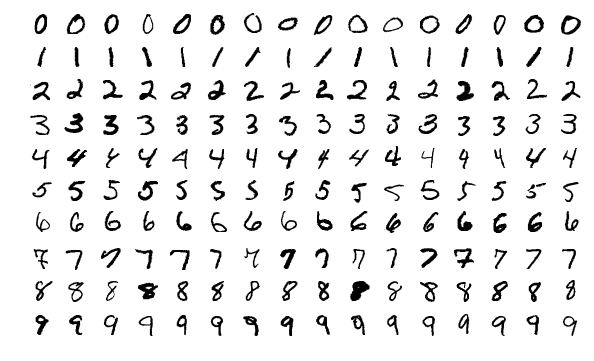
\includegraphics[width=200pt]{MnistExamples.png}
\caption{Esempi MNIST~\cite{pict_mnist}}
\end{center}
\label{fig:mnist}
\end{figure}

\subsection{Addestramento e tuning parametri}
\label{modselmnist}
Per trovare una buona configurazione della rete abbiamo effettuato una \textit{k-Fold Cross Validation}~\cite{Refaeilzadeh2009} con $k=3$. Abbiamo inoltre utilizzato la tecnica di dropout per mitigare gli effetti di un possibile overfitting durante il processo di apprendimento.
\paragraph*{K-Fold Cross Validation}
Il \textit{training set} viene diviso in \textit{k} sottoinsiemi, e a rotazione vengono usati come \textit{training set} $k-1$ sottoinsiemi, il rimanente sottoinsiemi viene usato come \textit{validation set}. Quest'ultimo serve per misurare la bontà della rete ottenuta fissando una configurazione dei parametri e addestrando sul training set. Alla fine si sceglie la rete che ha la bontà più alta e si usa il test set per valutare la capacità di generalizzazione.
\begin{figure}
\begin{center}
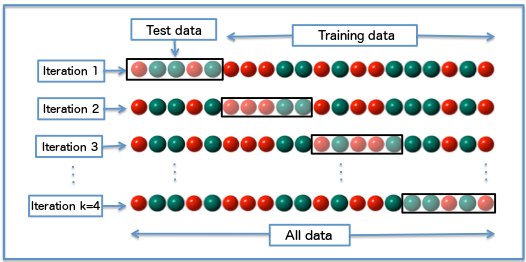
\includegraphics[width=300pt]{K-fold_cross_validation_EN.jpg}
\caption{Suddivisione di un dataset in un processo di cross validation a quattro fold~\cite{pict_kfold}}\label{fig:kfold}
\end{center}
\end{figure}
Nella Figura~\ref{fig:kfold} possiamo vedere un esempio di splitting del \textit{training set} con $k=4$.\\
Negli esperimenti abbiamo fissato i seguenti parametri:
\begin{itemize}
\item learning rate $\eta=3\times 10^{-3}$;
\item funzione errore: errore quadratico medio\footnote{$\frac{1}{n}\sum\limits^n_{i=1}{\left(t_i-y_i\right)}^2$, abbreviata negli ultimi esperimenti di questo capitolo con MSE};
\item metodo di apprendimento: discesa del gradiente con momentum ($\mu=0.99$);
\item funzione di attivazione degli strati \textit{hidden}: \textit{ReLU};
\item funzione di attivazione dello strato di output: \textit{softmax}\footnote{La funzione softmax è definita come $\text{softmax}(a_{i}) = \frac{\exp^{a_i}}{\sum_j \exp^{a_j}}$};
\item dimensione dei minibatch: 100 elementi;
\item criterio di arresto: 100 epoche;
\item inizializzazione dei pesi: generazione di numeri casuali (in particolare, ogni peso dello strato $l$ è impostato a $z \sqrt{2 / \mathrm{size}^{l-1}}$, dove $z$ è un valore pseudocasuale estratto da una distribuzione normale standard e $\mathrm{size}^{l-1}$ indica il numero di neuroni nello strato precedente\footnote{He et al initialization~\cite{he2015delving}}. 

\end{itemize}

I parametri di cui vogliamo trovare i valori migliori sono invece:
\begin{itemize}
\item architettura della rete (ovvero quanti strati hidden e quanti neuroni per ogni strato hidden);
\item dropout (percentuale di neuroni negli strati hidden non utilizzati nella fase di training).
\end{itemize}

\paragraph*{Dropout}
\begin{figure}
\begin{center}
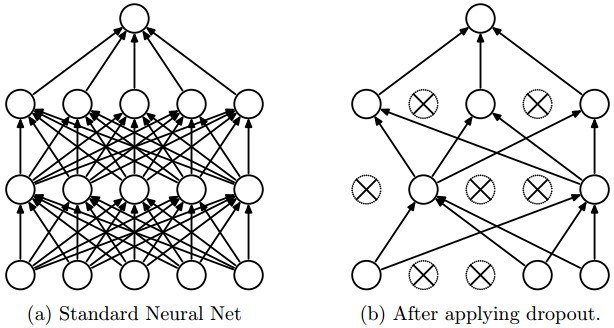
\includegraphics[width=200pt]{dropout.jpeg}
\caption{Visualizzazione della tecnica di dropout. (a) struttura di una rete neurale a tre strati. (b) modifica temporanea della struttura della rete durante un'iterazione dell'algoritmo di apprendimento, in cui i neuroni indicati con una croce non concorrono all'aggiornamento dei pesi della rete.~\cite{10.5555/2627435.2670313}} \label{fig:dropout}
\end{center}
\end{figure}
Il \textit{dropout}~\cite{10.5555/2627435.2670313} è una tecnica utilizzata per evitare l'overfitting mediante l'eliminazione casuale di alcuni neuroni in ogni strato, a eccezione di quello di output. I neuroni da eliminare cambiano a ogni epoca, durante la fase di predizione invece sono tutti attivi. Nella Figura~\ref{fig:dropout} possiamo vedere un esempio di questa tecnica.
Nell'elaborato è stata utilizzata la versione chiamata \textit{inverted dropout}
\begin{equation}
\mathrm{drop_l}=(\mathrm{rand} < p)/p,  \qquad
\mathrm{output_l}=\mathrm{output_l} * \mathrm{drop_l},
\label{drop}
\end{equation}
dove:
\begin{itemize}
\item $\mathrm{output_l}$ rappresenta l'output di un generico strato $l$
\item $\mathrm{rand}$ denota una matrice di numeri casuali estratti da una distribuzione uniforme nell'intervallo $[0,1)$ delle stesse dimensioni di $\mathrm{output_l}$,
\item $p$ rappresenta la probabilità di tenere attivo un neurone,
\item $*$ indica l'operatore di prodotto componente per componente tra due vettori.
\end{itemize} 
Nelle Tabelle~\ref{tab:modselmnist} e~\ref{tab:modselmnist2} sono indicati i risultati. Negli esperimenti effettuati abbiamo trovato come configurazione ottimale una rete MLP con uno strato hidden da 300 neuroni senza dropout (indicato nell'intestazione della tabella come $p=1$) che è anche la configurazione che abbiamo adottato negli esperimenti descritti di seguito.
\vspace*{\fill}
\begin{center}

\begin{table}[]
  \small
  \caption{Risultati della model selection per un MLP con uno strato hidden. La colonna \texttt{neuroni} indica il numero di neuroni nello strato hidden, la colonna \texttt{accuratezza} indica  la media delle accuratezze sui tre \textit{validation set}, mentre $p$ denota la probabilità di tenere attivo un generico neurone durante la fase di dropout. In grassetto è evidenziata la configurazione migliore.}\label{tab:modselmnist}
\begin{center}
\begin{tabular}{@{}cc|c@{}}

\hline\\[-11pt]
\hline\\[-6.5pt]
& $p=0.75$ & $p=1$ \\[5pt]
\hline\\[-11pt]
\texttt{neuroni} & \multicolumn{2}{c}{\texttt{accuratezza}} \\[1pt]
$100$ & $97.64$ & $97.38$ \\ [1pt]
$125$ & $97.63$ & $97.57$ \\ [1pt]
$150$ & $97.72$ & $94.41$ \\ [1pt]
$175$ & $97.75$ & $97.81$ \\ [1pt]
$200$ & $97.83$ & $94.29$ \\ [1pt]
$225$ & $97.82$ & $94.75$ \\ [1pt]
$250$ & $97.82$ & $94.88$ \\ [1pt]
$275$ & $97.84$ & $95.25$ \\ [1pt]
$300$ & $97.86$ & $\textbf{98.08}$ \\ [1pt]
\hline\\[-11pt]
\hline\\[-8pt]
\end{tabular}\\[5pt]
\end{center}
\normalsize
\end{table}
\end{center}

\vspace*{\fill}
\begin{center}

\begin{table}[]
  \small
  \caption{Risultati della model selection per un MLP con due strati hidden. Stesse notazioni della Tabella~\ref{tab:modselmnist} a eccezione della colonna \texttt{neuroni} che rappresenta il numero di neuroni dei due strati hidden.}\label{tab:modselmnist2}
\begin{center}
\begin{tabular}{cc|c||cc|c}
\hline\\[-11pt]
\hline\\[-6.5pt]
& $p=0.75$ & $p=1$ & & $p=0.75$ & $p=1$ \\[5pt]
\hline\\[-11pt]
\texttt{neuroni} & \multicolumn{2}{c}{\texttt{accuratezza}} & \texttt{neuroni} & \multicolumn{2}{c}{\texttt{accuratezza}} \\[1pt]
$50$ - $25$   & $97.14$ & $97.08$ &  $175$ - $125$ & $97.85$ & $97.80$ \\ [1pt]
$50$ - $50$   & $97.26$ & $96.82$ &  $175$ - $150$ & $97.82$ & $97.86$ \\ [1pt]
$75$ - $25$   & $97.43$ & $97.43$ &  $175$ - $175$ & $97.85$ & $97.84$ \\ [1pt]
$75$ - $50$   & $97.52$ & $97.51$ &  $200$ - $50$  & $97.83$ & $97.83$ \\ [1pt]
$75$ - $75$   & $97.51$ & $97.49$ &  $200$ - $75$  & $97.83$ & $97.90$ \\ [1pt]
$100$ - $25$  & $97.53$ & $97.54$ &  $200$ - $100$ & $97.88$ & $97.89$ \\ [1pt]
$100$ - $50$  & $97.66$ & $97.62$ &  $200$ - $125$ & $97.91$ & $97.85$ \\ [1pt]
$100$ - $75$  & $97.62$ & $97.63$ &  $200$ - $150$ & $97.84$ & $97.85$ \\ [1pt]
$100$ - $100$ & $97.67$ & $97.67$ &  $200$ - $175$ & $97.84$ & $97.89$ \\ [1pt]
$125$ - $25$  & $97.68$ & $97.62$ &  $200$ - $200$ & $97.86$ & $97.83$ \\ [1pt]
$125$ - $50$  & $97.77$ & $97.70$ &  $225$ - $75$  & $97.92$ & $97.90$ \\ [1pt]
$125$ - $75$  & $97.72$ & $97.68$ &  $225$ - $100$ & $97.86$ & $97.79$ \\ [1pt]
$125$ - $100$ & $97.73$ & $97.74$ &  $225$ - $125$ & $97.85$ & $97.85$ \\ [1pt]
$125$ - $125$ & $97.74$ & $97.77$ &  $225$ - $150$ & $97.94$ & $97.94$ \\ [1pt]
$150$ - $50$  & $97.71$ & $97.80$ &  $225$ - $175$ & $97.88$ & $97.89$ \\ [1pt]
$150$ - $75$  & $97.76$ & $97.76$ &  $225$ - $200$ & $97.91$ & $97.90$ \\ [1pt]
$150$ - $100$ & $97.75$ & $97.85$ &  $250$ - $75$  & $97.86$ & $97.88$ \\ [1pt]
$150$ - $125$ & $97.78$ & $97.74$ &  $250$ - $100$ & $97.91$ & $97.91$ \\ [1pt]
$150$ - $150$ & $97.75$ & $97.80$ &  $250$ - $125$ & $97.93$ & $97.94$ \\ [1pt]
$175$ - $50$  & $97.85$ & $97.80$ &  $250$ - $150$ & $97.93$ & $97.90$ \\ [1pt]
$175$ - $75$  & $97.80$ & $97.80$ &  $250$ - $175$ & $97.86$ & $97.90$ \\ [1pt]
$175$ - $100$ & $97.83$ & $97.80$ &  $250$ - $200$ & $97.89$ & $97.92$ \\ [1pt]

\hline\\[-11pt]
\hline\\[-8pt]
\end{tabular}\\[5pt]
\end{center}
\normalsize
\end{table}
\end{center}
\subsection{Pruning}
\label{pruningmnist}
Applicando la tecnica di pruning alla rete ottenuta dopo la procedura di model selection descritta nel paragrafo precedente abbiamo ottenuto i risultati descritti nella Tabella~\ref{tab:tabprmnist}. In particolare abbiamo applicato un pruning dal $10\%$ al $95\%$ a passi di $5\%$. Nella prima riga della Tabella~\ref{tab:tabprmnist} abbiamo riportato l'accuratezza sul \textit{test set} del modello scelto nel paragrafo precedente senza compressioni. Questi risultati da un lato mostrano come nonostante la rimozione di numerose connessioni (fino al 80\%) la rete appresa sia in grado di raggiungere accuratezze maggiori rispetto a quella della rete che le usa tutte; dall'altro lato, che la rete iniziale era sovradimensionata per il problema.
\vspace*{\fill}
\begin{center}
\begin{table}[]
  \small
  \caption{Variazione dell'accuratezza della rete che ha appreso a classificare le cifre MNIST applicando la tecnica di pruning}\label{tab:tabprmnist}
\begin{center}
\begin{tabular}{ccc|ccc}

\hline\\[-11pt]

\hline\\[-11pt]
\texttt{pruning \%} & \texttt{accuratezza} & $r_1$ & \texttt{pruning \%} & \texttt{accuratezza} & $r_1$ \\[1pt]
\hline\\[-6.5pt]
ALL    & $98.34$ &    & $55\%$ & $98.32$ & 0.9\\ 
$10\%$ & $98.34$ &$1.8$ & $60\%$ & $98.30$ & $0.8$\\ 
$15\%$ & $98.34$ &$1.7$ & $65\%$ & $98.33$ & $0.7$\\ 
$20\%$ & $98.34$ &$1.6$ & $70\%$ & $98.34$ & $0.6$\\ 
$25\%$ & $98.35$ &$1.5$ & $75\%$ & $98.34$ & $0.5$\\ 
$30\%$ & $98.36$ &$1.4$ & $80\%$ & $98.38$ & $0.4$\\ 
$35\%$ & $98.35$ &$1.3$ & $85\%$ & $98.31$ & $0.3$\\ 
$40\%$ & $98.36$ &$1.2$ & $90\%$ & $98.27$ & $0.2$\\ 
$45\%$ & $98.36$ &$1.1$ & $95\%$ & $98.28$ & $0.1$\\ 
$50\%$ & $98.36$ &$1.0$&&&\\  
\hline\\[-11pt]
\hline\\[-8pt]
\end{tabular}\\[5pt]
\end{center}
\normalsize
\end{table}
\end{center}
\subsection{Weight sharing}
La Tabella~\ref{tab:tabwsmnist} riporta i risultati dell'applicazione della tecnica di weight sharing alla rete ottenuta nel Paragrafo~\ref{modselmnist}. La prima colonna rappresenta il numero di centroidi utilizzati per la compressione, specificati separatamente per i due strati della rete. Nella prima riga della Tabella~\ref{tab:tabwsmnist} abbiamo riportato l'accuratezza sul \textit{test set} del modello scelto senza compressioni. Come avvenuto con il pruning, possiamo notare che l'accuratezza rimane sopra il 98\% anche considerando un numero abbastanza piccolo di centroidi.
Nella colonna $r_2$ possiamo notare valori molto vicini al variare dei cluster, riprendendo~\eqref{tassows}: $s$ (che ricordiamo essere il prodotto delle dimensioni della matrice) è sempre maggiore di 256, quindi $f(s)=16$; semplificando la formula troviamo $$\displaystyle{\frac{1}{2}+\frac{k}{s}},$$ per questo motivo $r_2$ non può essere minore di $0.5$.
\vspace*{\fill}
\begin{center}
\begin{table}[]
  \small
  \caption{Variazione dell'accuratezza della rete che ha appreso a classificare le cifre MNIST applicando la tecnica di weight sharing}\label{tab:tabwsmnist}
\begin{center}
\begin{tabular}{ccc|ccc}

\hline\\[-11pt]

\hline\\[-11pt]
\texttt{centroidi} & \texttt{accuratezza} & $r_2$ & \texttt{centroidi} & \texttt{accuratezza} & $r_2$ \\[1pt]
\hline\\[-6.5pt]
ALL          & $98.34$ &       & $256$ - $64$  & $98.36$ & $0.5$\\ 
$4$ - $2$    & $94.00$ & $0.5$ & $512$ - $32$  & $98.38$ & $0.5$\\   
$16$ - $8$   & $98.14$ & $0.5$ & $512$ - $64$  & $98.35$ & $0.5$\\ 
$32$ - $8$   & $98.32$ & $0.5$ & $1024$ - $32$ & $98.37$ & $0.5$\\   
$32$ - $16$  & $98.25$ & $0.5$ & $1024$ - $64$ & $98.37$ & $0.5$\\ 
$64$ - $16$  & $98.29$ & $0.5$ & $2048$ - $32$ & $98.36$ & $0.51$\\   
$64$ - $32$  & $98.34$ & $0.5$ & $2048$ - $64$ & $98.36$ & $0.51$\\ 
$128$ - $32$ & $98.38$ & $0.5$ & $4096$ - $32$ & $98.35$ & $0.52$\\  
$192$ - $32$ & $98.38$ & $0.5$ & $4096$ - $64$ & $98.37$ & $0.52$\\  
$192$ - $64$ & $98.36$ & $0.5$ & $8192$ - $32$ & $98.43$ & $0.53$\\
$256$ - $32$ & $98.31$ & $0.5$ & $8192$ - $64$ & $98.34$ & $0.53$\\  
\hline\\[-11pt]
\hline\\[-8pt]
\end{tabular}\\[5pt]
\end{center}
\normalsize
\end{table}
\end{center}

\section{Problema del predecessore}
Fissato un universo $U$, sul quale è definita una relazione di ordine totale $\leq$, consideriamo un sottoinsieme $X \subseteq U$ i cui elementi chiameremo \emph{chiavi}. Il problema di ricerca del predecessore consiste nel trovare la posizione della chiave più grande in $X$ che non sia maggiore di un valore $x$ dato in input. Se per ogni $x \in X$ indichiamo con $\mathrm{pos}(x)$ la posizione di $x$ nella sequenza ottenuta ordinando gli elementi di $X$, il problema equivale a determinare il valore $\mathrm{pred}(x) = \mathrm{pos}(z)$, dove $z = arg max{y \in X} \{ y \leq x\}$.
Se per esempio consideriamo l'insieme $$\displaystyle{ X=\{2,3,4,5,12,15,18\}}$$ e assumiamo $x=7$, la ricerca del predecessore dovrebbe restituire la posizione 4.

Dato $|X|=n$, sia $F_X: U \mapsto [0, 1]$ la distribuzione cumulativa empirica degli elementi di $U$ rispetto a $X$, per ogni $x\in U$, $F_X(x) = \frac{| \{x' \in X \text{ tale che }x' \leq x\} |}{n}$. Per semplificare la notazione, denotiamo $F_{X}$ con $F$. Nell'esempio sopra indicato, si avrà dunque $F(2)=\frac{1}{7}$, $F(5)=\frac{4}{7}$, $F(6)=\frac{4}{7}$, $F(18)=1$. La conoscenza di $F$ ci dà una soluzione al nostro problema, in quanto dato un generico $x \in U$, una sola valutazione di $F$ fornisce $\mathrm{pred}(x) = \ceil{(F(z)\cdot n)}$. Il nostro obiettivo è quindi quello di trovare una rete neurale che calcoli una buona approssimazione $\tilde{F}$ di $F$.
La risoluzione di questo problema potrebbe consentire di trovare un elemento all'interno di una lista ordinata in tempo $O(1)$ invece che $O(\log n)$ tipico degli alberi binari di ricerca.
La rete neurale però può compiere un errore nel dare la posizione di un elemento, per questo motivo teniamo traccia dell'errore massimo, indicato con $\epsilon$, che la rete compie. Pertanto durante la ricerca, dopo che il modello ha predetto la posizione, dovremo effettuare una ricerca che coinvolgerà al più $\epsilon$ posizioni a destra e a sinistra rispetto a quanto indicato dal modello. Per questo motivo, dopo aver utilizzato delle funzioni di errore standard (come l'errore quadratico medio) che minimizzano l'errore medio, negli esperimenti abbiamo provato ad allenare la rete neurale minimizzando una funzione convessa che approssima il massimo. Tale funzione prende il nome di $\mathrm{LogSumExp}$ è descritta nel Paragrafo~\ref{seclse}.

Per questo problema sono stati utilizzati tre dataset, rispettivamente con $512$, $8192$ e $1048576$ esempi. Questi dataset saranno successivamente indicati rispettivamente come dataset 3, dataset 7 e dataset 10.
Diversamente da MNIST, il modello MLP cercherà di risolvere un problema di regressione: la rete neurale dovrà imparare a restituire, data una chiave, il corrispondente valore di $\tilde{F}$.
Sono state usate tre reti differenti:
\begin{itemize}
\item{rete 1 con zero strati hidden};
\item{rete 2 con uno strato hidden di 256 neuroni};
\item{rete 3 con due strati hidden di 256 neuroni}.
\end{itemize}
Per tutte e tre le reti, dove non indicato esplicitamente, i parametri utilizzati sono:
\begin{itemize}
\item funzione errore: errore quadratico medio;
\item metodo di apprendimento: discesa del gradiente con momentum ($\mu=0.9$);
\item funzione di attivazione dei neuroni: \textit{LeakyReLU} ($\alpha=0.05$);
\item{$\lambda$} = $10^{-5}$ \footnote{usato per nella regolarizzazione l2, valore aggiunto alla funzione di errore che penalizza i pesi più grandi, riducendo così il problema di overfitting ~\cite{L2}.};
\item{dimensione dei minibatch}: $64$;
\item{epoche}: $20000$;
\item{criterio di arresto}: l'apprendimento termina se non si hanno miglioramenti di performance con $\textit{patience}=4$ (vedi Paragrafo~\ref{stopping});
\item inizializzazione dei pesi = numeri casuali estratti da una distribuzione normale con $\mu=0$ e $\sigma= 0.05$. 
\end{itemize}
Ci riferiremo a queste reti con NNX, dove X indica il numero totale di strati (compreso quello di output).
Per NN1 è stato usato un learning rate $\eta=5 \times 10^{-4}$, mentre per NN2 e NN3 si ha $\eta=3 \times 10^{-3}$. Questi valori sono stati trovati eseguendo un tuning su $\eta$.

I risultati ottenuti sono indicati nelle Tabelle~\ref{pr13} -~\ref{ws310}, che riportano le seguenti colonne:
\begin{itemize}
\item Pruning \%: percentuale di connessioni eliminate (calcolate sulla base di quantili come indicato nel Paragrafo\ref{percentile}); in particolare, 0 indica la rete non compressa;
\item $r_2$: proporzione dello spazio originario occupato da quella compressa (1 indica la rete non compressa);
\item Clusters: numero di cluster utilizzati per ogni matrice dei pesi;
\item Space Overhead (KB):  spazio del modello (in KB) rispetto al dataset, calcolata come $$\displaystyle{\frac{\sum\limits_{i=1}^n \left(|\mathrm{strato}_i|\right) \cdot \mathrm{bytes} \cdot 100}{1024 \cdot \left| \mathrm{dataset} \right|}}$$ dove per $\mathrm{strato}_i$ viene preso in considerazione il prodotto delle dimensioni della matrice delle connessioni per memorizzare i pesi per l'$i$-esimo strato, bytes rappresenta il numero di bytes utilizzato per rappresentare i pesi;
\item Training Time (s): tempo (in secondi) impiegato dalla rete per il training, compreso il tempo iniziale di applicazione della compressione (nella rete non compressa non viene indicato questo tempo, questi casi sono indicati con -);
\item $\epsilon$: errore massimo sugli esempi di training;
\item Error \%: errore massimo rispetto alla dimensione del dataset considerato;
\item Mean Error: errore medio.
\end{itemize}

\subsection{Pruning}
\label{prpred}
Le Tabelle~\ref{pr13} -~\ref{pr310} mostrano i risultati dell'applicazione della tecnica di pruning alle reti ottenute per il problema del predecessore. Come accennato nel Paragrafo~\ref{sectassopr} prima di raggiungere una certa sparsità il modello compresso occupa più spazio del modello originario. I modelli compressi occupano meno spazio a partire da una percentuale di pruning compresa tra il 50\% e il 60\%.
Nei risultati di questi esperimenti possiamo notare una scarsa efficacia del pruning in reti con pochi neuroni (NN1), mentre (come già visto con MNIST nel Paragrafo~\ref{pruningmnist}) con molti neuroni (NN2 e NN3) il pruning a percentuali molto elevate mantiene errori medi ed errori massimi equivalenti alla rete non compressa, se non migliori. 
Infatti sul dataset 10 si riesce ad arrivare a tassi di compressione maggiori, fino a 80\%, migliorando l'errore. Possiamo osservare che, per la natura del problema (le posizioni rapprentano una successione monotona non decrescente), la rete NN1 risulta milgiore per questo problema (il rapporto prestazioni/spazio è sempre a suo favore).
\begin{adjustwidth}{0cm}{}
\begin{table}
\caption{NN1 dataset 3}\label{pr13}
\begin{tabular}{cccccc}
\hline
%\multicolumn{6}{c}{NN1 dataset 3} \\
\toprule
Pruning \% & Space Overhead (KB) & Training Time (s) & $\epsilon$ & Error \% & Mean Error\\
\midrule
$0$ & $8.93 \times 10^{-2}$ & - & $9$ & $1.76$ & $4.74 \times 10^{-3}$\\
$10$ & $8.56 \times 10^{-2}$ & $7.0 \times 10^{-3}$ & $8$ & $1.56$ & $4.58 \times 10^{-3}$\\
$20$ & $8.01 \times 10^{-2}$ & $7.6 \times 10^{-3}$ & $8$ & $1.56$ & $4.58 \times 10^{-3}$\\
$30$ & $7.10 \times 10^{-2}$ & $7.5 \times 10^{-3}$ & $8$ & $1.56$ & $4.59 \times 10^{-3}$\\
$40$ & $6.03 \times 10^{-2}$ & $7.2 \times 10^{-3}$ & $9$ & $1.76$ & $4.82 \times 10^{-3}$\\
$50$ & $5.11 \times 10^{-2}$ & $8.9 \times 10^{-3}$ & $14$ & $2.73$ & $8.91 \times 10^{-3}$\\
$60$ & $4.20 \times 10^{-2}$ & $8.9 \times 10^{-3}$ & $21$ & $4.1$ & $1.60 \times 10^{-2}$\\
$70$ & $3.13 \times 10^{-2}$ & $1.2 \times 10^{-2}$ & $36$ & $7.03$ & $3.13 \times 10^{-2}$\\
$80$ & $2.21 \times 10^{-2}$ & $1.1 \times 10^{-2}$ & $66$ & $1.28 \times 10$ & $6.25 \times 10^{-2}$\\
$90$ & $1.30 \times 10^{-2}$ & $1.1 \times 10^{-2}$ & $65$ & $1.27 \times 10$ & $6.25 \times 10^{-2}$\\
\bottomrule
\end{tabular}
\end{table}
\end{adjustwidth}

\begin{adjustwidth}{0cm}{}
\begin{table}
\caption{NN1 dataset 7}\label{pr17}
\begin{tabular}{cccccc}
\hline
%\multicolumn{6}{c}{NN1 dataset 7} \\
\toprule
Pruning \% & Space Overhead (KB) & Training Time (s) & $\epsilon$ & Error \% & Mean Error\\
\midrule
$0$ & $3.09 \times 10^{-3}$ & - & $53$ & $6.4 \times 10^{-1}$ & $1.62 \times 10^{-3}$\\
$10$ & $5.58 \times 10^{-3}$ & $8.1 \times 10^{-2}$ & $46$ & $5.6 \times 10^{-1}$ & $1.55 \times 10^{-3}$\\
$20$ & $5.01 \times 10^{-3}$ & $8.1 \times 10^{-2}$ & $43$ & $5.2 \times 10^{-1}$ & $1.52 \times 10^{-3}$\\
$30$ & $4.43 \times 10^{-3}$ & $8.9 \times 10^{-2}$ & $44$ & $5.4 \times 10^{-1}$ & $1.53 \times 10^{-3}$\\
$40$ & $3.77 \times 10^{-3}$ & $9.3 \times 10^{-2}$ & $55$ & $6.7 \times 10^{-1}$ & $1.77 \times 10^{-3}$\\
$50$ & $3.19 \times 10^{-3}$ & $1.2 \times 10^{-1}$ & $73$ & $8.9 \times 10^{-1}$ & $2.41 \times 10^{-3}$\\
$60$ & $2.62 \times 10^{-3}$ & $1.2 \times 10^{-1}$ & $107$ & $1.31$ & $4.17 \times 10^{-3}$\\
$70$ & $1.96 \times 10^{-3}$ & $1.7 \times 10^{-1}$ & $107$ & $1.31$ & $4.17 \times 10^{-3}$\\
$80$ & $1.38 \times 10^{-3}$ & $2.4 \times 10^{-1}$ & $165$ & $2.01$ & $7.97 \times 10^{-3}$\\
$90$ & $8.11 \times 10^{-4}$ & $2.2 \times 10^{-1}$ & $165$ & $2.01$ & $7.97 \times 10^{-3}$\\
\bottomrule
\end{tabular}
\end{table}
\end{adjustwidth}

\begin{adjustwidth}{0cm}{}
\begin{table}
\caption{NN1 dataset 10}\label{pr110}
\begin{tabular}{cccccc}
\hline
%\multicolumn{6}{c}{NN1 dataset 10} \\
\toprule
Pruning \% & Space Overhead (KB) & Training Time (s) & $\epsilon$ & Error \% & Mean Error\\
\midrule
$0$ & $2.42 \times 10^{-5}$ & - & $905$ & $8.6 \times 10^{-2}$ & $1.85 \times 10^{-4}$\\
$10$ & $4.35 \times 10^{-5}$ & $1.1 \times 10$ & $770$ & $7 \times 10^{-2}$ & $1.52 \times 10^{-4}$\\
$20$ & $3.91 \times 10^{-5}$ & $1.6 \times 10$ & $770$ & $7 \times 10^{-2}$ & $1.52 \times 10^{-4}$\\
$30$ & $3.46 \times 10^{-5}$ & $1.1 \times 10$ & $770$ & $7 \times 10^{-2}$ & $1.52 \times 10^{-4}$\\
$40$ & $2.94 \times 10^{-5}$ & $1.1 \times 10$ & $770$ & $7 \times 10^{-2}$ & $1.52 \times 10^{-4}$\\
$50$ & $2.49 \times 10^{-5}$ & $1.4 \times 10$ & $770$ & $7 \times 10^{-2}$ & $1.52 \times 10^{-4}$\\
$60$ & $2.05 \times 10^{-5}$ & $1.2 \times 10$ & $734$ & $7 \times 10^{-2}$ & $1.50 \times 10^{-4}$\\
$70$ & $1.53 \times 10^{-5}$ & $1.1 \times 10$ & $736$ & $7 \times 10^{-2}$ & $1.51 \times 10^{-4}$\\
$80$ & $1.08 \times 10^{-5}$ & $1.1 \times 10$ & $748$ & $7 \times 10^{-2}$ & $1.51 \times 10^{-4}$\\
$90$ & $6.32 \times 10^{-6}$ & $1.1 \times 10$ & $5235$ & $4.9 \times 10^{-1}$ & $1.97 \times 10^{-4}$\\
\bottomrule
\end{tabular}
\end{table}
\end{adjustwidth}

\begin{adjustwidth}{0cm}{}
\begin{table}
\caption{NN2 dataset 3}\label{pr23}
\begin{tabular}{cccccc}
\hline
%\multicolumn{6}{c}{NN2 dataset 3} \\
\toprule
Pruning \% & Space Overhead (KB) & Training Time (s) & $\epsilon$ & Error \% & Mean Error\\
\midrule
$0$ & $1.289 \times 10$ & - & $4$ & $7.8 \times 10^{-1}$ & $1.60 \times 10^{-3}$\\
$10$ & $2.324 \times 10$ & $2.1 \times 10$ & $2$ & $3.9 \times 10^{-1}$ & $6.12 \times 10^{-4}$\\
$20$ & $2.070 \times 10$ & $2.3 \times 10$ & $2$ & $3.9 \times 10^{-1}$ & $6.21 \times 10^{-4}$\\
$30$ & $1.817 \times 10$ & $2.1 \times 10$ & $3$ & $5.8 \times 10^{-1}$ & $6.93 \times 10^{-4}$\\
$40$ & $1.563 \times 10$ & $2.0 \times 10$ & $3$ & $5.8 \times 10^{-1}$ & $7.93 \times 10^{-4}$\\
$50$ & $1.309 \times 10$ & $2.1 \times 10$ & $3$ & $5.8 \times 10^{-1}$ & $8.62 \times 10^{-4}$\\
$60$ & $1.055 \times 10$ & $2.3 \times 10$ & $3$ & $5.8 \times 10^{-1}$ & $9.85 \times 10^{-4}$\\
$70$ & $8.01$ & $2.1 \times 10$ & $4$ & $7.8 \times 10^{-1}$ & $1.32 \times 10^{-3}$\\
$80$ & $5.47$ & $1.7 \times 10$ & $5$ & $9.7 \times 10^{-1}$ & $1.95 \times 10^{-3}$\\
$90$ & $2.93$ & $1.2 \times 10$ & $6$ & $1.17$ & $2.78 \times 10^{-3}$\\
\bottomrule
\end{tabular}
\end{table}
\end{adjustwidth}

\begin{adjustwidth}{0cm}{}
\begin{table}
\caption{NN2 dataset 7}\label{pr27}
\begin{tabular}{cccccc}
\hline
%\multicolumn{6}{c}{NN2 dataset 7} \\
\toprule
Pruning \% & Space Overhead (KB) & Training Time (s) & $\epsilon$ & Error \% & Mean Error\\
\midrule
$0$ & $8.06 \times 10^{-1}$ & - & $33$ & $4.0 \times 10^{-1}$ & $1.12 \times 10^{-3}$\\
$10$ & $1.45$ & $1.31 \times 10^{2}$ & $35$ & $4.3 \times 10^{-1}$ & $5.94 \times 10^{-4}$\\
$20$ & $1.29$ & $1.23 \times 10^{2}$ & $35$ & $4.3 \times 10^{-1}$ & $5.98 \times 10^{-4}$\\
$30$ & $1.13$ & $1.18 \times 10^{2}$ & $35$ & $4.3 \times 10^{-1}$ & $6.04 \times 10^{-4}$\\
$40$ & $9.76 \times 10^{-1}$ & $1.18 \times 10^{2}$ & $35$ & $4.3 \times 10^{-1}$ & $5.97 \times 10^{-4}$\\
$50$ & $8.18 \times 10^{-1}$ & $1.15 \times 10^{2}$ & $34$ & $4.2 \times 10^{-1}$ & $5.99 \times 10^{-4}$\\
$60$ & $6.59 \times 10^{-1}$ & $1.11 \times 10^{2}$ & $35$ & $4.3 \times 10^{-1}$ & $6.11 \times 10^{-4}$\\
$70$ & $5.00 \times 10^{-1}$ & $1.24 \times 10^{2}$ & $35$ & $4.3 \times 10^{-1}$ & $6.12 \times 10^{-4}$\\
$80$ & $3.42 \times 10^{-1}$ & $2.2 \times 10$ & $33$ & $4.0 \times 10^{-1}$ & $8.56 \times 10^{-4}$\\
$90$ & $1.83 \times 10^{-1}$ & $5$ & $34$ & $4.1 \times 10^{-1}$ & $1.19 \times 10^{-3}$\\
\bottomrule
\end{tabular}
\end{table}
\end{adjustwidth}

\begin{adjustwidth}{0cm}{}
\begin{table}
\caption{NN2 dataset 10}\label{pr210}
\begin{tabular}{cccccc}
\hline
%\multicolumn{6}{c}{NN2 dataset 10} \\
\toprule
Pruning \% & Space Overhead (KB) & Training Time (s) & $\epsilon$ & Error \% & Mean Error\\
\midrule
$0$ & $6.29 \times 10^{-3}$ & - & $1031$ & $9.0 \times 10^{-2}$ & $2.33 \times 10^{-4}$\\
$10$ & $1.13 \times 10^{-2}$ & $1.74 \times 10^{2}$ & $713$ & $6.8 \times 10^{-2}$ & $1.46 \times 10^{-4}$\\
$20$ & $1.01 \times 10^{-2}$ & $1.25 \times 10^{2}$ & $713$ & $6.8 \times 10^{-2}$ & $1.46 \times 10^{-4}$\\
$30$ & $8.87 \times 10^{-3}$ & $1.25 \times 10^{2}$ & $713$ & $6.8 \times 10^{-2}$ & $1.46 \times 10^{-4}$\\
$40$ & $7.63 \times 10^{-3}$ & $1.24 \times 10^{2}$ & $713$ & $6.8 \times 10^{-2}$ & $1.46 \times 10^{-4}$\\
$50$ & $6.39 \times 10^{-3}$ & $1.22 \times 10^{2}$ & $713$ & $6.8 \times 10^{-2}$ & $1.46 \times 10^{-4}$\\
$60$ & $5.15 \times 10^{-3}$ & $1.22 \times 10^{2}$ & $713$ & $6.8 \times 10^{-2}$ & $1.46 \times 10^{-4}$\\
$70$ & $3.91 \times 10^{-3}$ & $1.22 \times 10^{2}$ & $713$ & $6.8 \times 10^{-2}$ & $1.46 \times 10^{-4}$\\
$80$ & $2.67 \times 10^{-3}$ & $1.22 \times 10^{2}$ & $715$ & $6.8 \times 10^{-2}$ & $1.46 \times 10^{-4}$\\
$90$ & $1.43 \times 10^{-3}$ & $1.23 \times 10^{2}$ & $699$ & $6.7 \times 10^{-2}$ & $1.45 \times 10^{-4}$\\
\bottomrule
\end{tabular}
\end{table}
\end{adjustwidth}

\begin{adjustwidth}{0cm}{}
\begin{table}
\caption{NN3 dataset 3}\label{pr33}
\begin{tabular}{cccccc}
\hline
%\multicolumn{6}{c}{NN3 dataset 3} \\
\toprule
Pruning \% & Space Overhead (KB) & Training Time (s) & $\epsilon$ & Error \% & Mean Error\\
\midrule
$0$ & $6.308 \times 10$ & - & $4$ & $7.8$ & $1.83 \times 10^{-3}$\\
$10$ & $1.13 \times 10^2 $ & $6.1 \times 10$ & $2$ & $3.9 \times 10^{-1}$ & $6.63 \times 10^{-4}$\\
$20$ & $1.01 \times 10^2 $ & $6.3 \times 10$ & $2$ & $3.9 \times 10^{-1}$ & $6.86 \times 10^{-4}$\\
$30$ & $8.855 \times 10$ & $5.6 \times 10$ & $2$ & $3.9 \times 10^{-1}$ & $7.66 \times 10^{-4}$\\
$40$ & $7.601 \times 10$ & $5.6 \times 10$ & $3$ & $5.8 \times 10^{-1}$ & $8.79 \times 10^{-4}$\\
$50$ & $6.348 \times 10$ & $6.6 \times 10$ & $3$ & $5.8 \times 10^{-1}$ & $8.82 \times 10^{-4}$\\
$60$ & $5.094 \times 10$ & $6.6 \times 10$ & $3$ & $5.8 \times 10^{-1}$ & $1.02 \times 10^{-3}$\\
$70$ & $3.840 \times 10$ & $7.1 \times 10$ & $3$ & $5.8 \times 10^{-1}$ & $1.15 \times 10^{-3}$\\
$80$ & $2.586 \times 10$ & $6.9 \times 10$ & $3$ & $5.8 \times 10^{-1}$ & $1.50 \times 10^{-3}$\\
$90$ & $1.332 \times 10$ & $8.1 \times 10$ & $4$ & $7.8 \times 10^{-1}$ & $2.03 \times 10^{-3}$\\
\bottomrule
\end{tabular}
\end{table}
\end{adjustwidth}

\begin{adjustwidth}{0cm}{}
\begin{table}
\caption{NN3 dataset 7}\label{pr37}
\begin{tabular}{cccccc}
\hline
%\multicolumn{6}{c}{NN3 dataset 7} \\
\toprule
Pruning \% & Space Overhead (KB) & Training Time (s) & $\epsilon$ & Error \% & Mean Error\\
\midrule
$0$ & $3.94$ & - & $40$ & $4.8 \times 10^{-1}$ & $1.14 \times 10^{-3}$\\
$10$ & $7.10$ & $1.97  \times 10^{2}$ & $36$ & $4.3 \times 10^{-1}$ & $7.80 \times 10^{-4}$\\
$20$ & $6.31$ & $2.27 \times 10^{2}$ & $36$ & $4.3 \times 10^{-1}$ & $7.58 \times 10^{-4}$\\
$30$ & $5.53$ & $9.5 \times 10$ & $32$ & $3.9 \times 10^{-1}$ & $8.18 \times 10^{-4}$\\
$40$ & $4.75$ & $1.04 \times 10^{2}$ & $33$ & $4.0 \times 10^{-1}$ & $8.18 \times 10^{-4}$\\
$50$ & $3.97$ & $9.6 \times 10$ & $33$ & $4.0 \times 10^{-1}$ & $8.23 \times 10^{-4}$\\
$60$ & $3.18$ & $1.25 \times 10^{2}$ & $34$ & $4.1 \times 10^{-1}$ & $8.12 \times 10^{-4}$\\
$70$ & $2.40$ & $9.9 \times 10$ & $34$ & $4.1 \times 10^{-1}$ & $8.29 \times 10^{-4}$\\
$80$ & $1.61$ & $9.3 \times 10$ & $34$ & $4.1 \times 10^{-1}$ & $8.20 \times 10^{-4}$\\
$90$ & $8.32 \times 10^{-1}$ & $2.9 \times 10$ & $32$ & $3.9 \times 10^{-1}$ & $1.24 \times 10^{-3}$\\
\bottomrule
\end{tabular}
\end{table}
\end{adjustwidth}

\begin{adjustwidth}{0cm}{}
\begin{table}
\caption{NN3 dataset 10}\label{pr310}
\begin{tabular}{cccccc}
\hline
%\multicolumn{6}{c}{NN3 dataset 10} \\
\toprule
Pruning \% & Space Overhead (KB) & Training Time (s) & $\epsilon$ & Error \% & Mean Error\\
\midrule
$0$ & $3.08 \times 10^{-2}$ & - & $1270$ & $1.2 \times 10^{-1}$ & $2.40 \times 10^{-4}$\\
$10$ & $5.54 \times 10^{-2}$ & $3.02 \times 10^{2}$ & $708$ & $6.8 \times 10^{-2}$ & $1.47 \times 10^{-4}$\\
$20$ & $4.93 \times 10^{-2}$ & $3.03 \times 10^{2}$ & $708$ & $6.8 \times 10^{-2}$ & $1.47 \times 10^{-4}$\\
$30$ & $4.32 \times 10^{-2}$ & $3.04 \times 10^{2}$ & $708$ & $6.8 \times 10^{-2}$ & $1.47 \times 10^{-4}$\\
$40$ & $3.71 \times 10^{-2}$ & $3.05 \times 10^{2}$ & $707$ & $6.8 \times 10^{-2}$ & $1.47 \times 10^{-4}$\\
$50$ & $3.09 \times 10^{-2}$ & $3.04 \times 10^{2}$ & $707$ & $6.7 \times 10^{-2}$ & $1.47 \times 10^{-4}$\\
$60$ & $2.49 \times 10^{-2}$ & $3.00 \times 10^{2}$ & $707$ & $6.7 \times 10^{-2}$ & $1.47 \times 10^{-4}$\\
$70$ & $1.87 \times 10^{-2}$ & $3.00 \times 10^{2}$ & $706$ & $6.7 \times 10^{-2}$ & $1.47 \times 10^{-4}$\\
$80$ & $1.26 \times 10^{-2}$ & $3.02 \times 10^{2}$ & $700$ & $6.7 \times 10^{-2}$ & $1.46 \times 10^{-4}$\\
$90$ & $6.50 \times 10^{-3}$ & $3.00 \times 10^{2}$ & $660$ & $6.3 \times 10^{-2}$ & $1.45 \times 10^{-4}$\\
\bottomrule
\end{tabular}
\end{table}
\end{adjustwidth}
\subsection{Weight Sharing}
Le Tabelle~\ref{ws13} -~\ref{ws310} mostrano i risultati dell'applicazione della tecnica di weight sharing alle reti ottenute per il problema del predecessore.
Il numero di centroidi è calcolato come
\begin{equation}
\mathrm{cluster}=\left(\frac{r_2 \times32s -sb}{32}\right)
\label{cluster}
\end{equation}
dove $r_2$ è il tasso di compressione (vedi Paragrafo~\ref{sec:tassows}), $s$ è il numero di connessioni e $b$ è il numero di byte utilizzati per rappresentare i centroidi.
Per~\eqref{cluster} e~\eqref{tassows} non possiamo raggiungere valori di $r_2$ inferiori a quelli mostrati nelle tabelle.
Come ci si aspetta, al crescere del numero di centroidi le reti hanno una performance crescente e in alcuni casi migliore della rete non compressa. Anche da questi esperimenti NN1 si fa preferire per prestazioni e spazio occupato.
\begin{adjustwidth}{-1cm}{}
\begin{table}
\caption{NN1 dataset 3}\label{ws13}
\begin{tabular}{ccccccc}
\hline
%\multicolumn{7}{c}{NN1 dataset 3} \\
\toprule
$r_2$ & Clusters & Space Overhead (KB) & Training Time (s) & $\epsilon$ & Error \% & Mean Error\\
\midrule
 & - & $4.95 \times 10^{-2}$ & - & $9$ & $1.75$ & $4.74 \times 10^{-3}$\\
$0.3$ & $3$ & $1.60 \times 10^{-2}$ & $8.07 \times 10^{-2}$ & $2427$ & $4.74 \times 10^2$ & $3.15$\\
$0.4$ & $9$ & $2.06 \times 10^{-2}$ & $8.69 \times 10^{-2}$ & $14373$ & $2.80 \times 10^3$ & $1.78 \times 10$\\
$0.5$ & $16$ & $2.59 \times 10^{-2}$ & $9.27 \times 10^{-2}$ & $5714$ & $1.11 \times 10^3$ & $7.32$\\
$0.6$ & $22$ & $3.05 \times 10^{-2}$ & $1.93 \times 10^{-1}$ & $5296$ & $1.03 \times 10^3$ & $6.80$\\
$0.7$ & $28$ & $3.51 \times 10^{-2}$ & $1.93 \times 10^{-1}$ & $8159$ & $1.59 \times 10^3$ & $1.03 \times 10$\\
$0.8$ & $35$ & $4.04 \times 10^{-2}$ & $2.08 \times 10^{-1}$ & $542$ & $1.05 \times 10^2$ & $5.83 \times 10^{-1}$\\
$0.9$ & $41$ & $4.50 \times 10^{-2}$ & $2.44 \times 10^{-1}$ & $8$ & $1.56$ & $4.60 \times 10^{-3}$\\
\bottomrule
\end{tabular}
\end{table}
\end{adjustwidth}

\begin{adjustwidth}{-1cm}{}
\begin{table}
\caption{NN1 dataset 7}\label{ws17}
\begin{tabular}{ccccccc}
\hline
%\multicolumn{7}{c}{NN1 dataset 7} \\
\toprule
$r_2$ & Clusters & Space Overhead (KB) & Training Time (s) & $\epsilon$ & Error \% & Mean Error\\
\midrule
& - & $3.09 \times 10^{-3}$ & - & $53$ & $6.47 \times 10^{-1}$ & $1.62 \times 10^{-3}$\\
$0.3$ & $3$ & $1.00 \times 10^{-3}$ & $2.71 \times 10^{-1}$ & $57 \times 10^7$ & $69.62 \times 10^5$ & $4.27 \times 10^3$\\
$0.4$ & $9$ & $1.29 \times 10^{-3}$ & $2.71 \times 10^{-1}$ & $37 \times 10^4$ & $46.34 \times 10^2$ & $2.71 \times 10$\\
$0.5$ & $16$ & $1.62 \times 10^{-3}$ & $3.02 \times 10^{-1}$ & $10 \times 10^4$ & $12.54 \times 10^2$ & $7.20$\\
$0.6$ & $22$ & $1.91 \times 10^{-3}$ & $3.55 \times 10^{-1}$ & $21 \times 10^4$ & $25.76 \times 10^2$ & $1.46 \times 10$\\
$0.7$ & $28$ & $2.19 \times 10^{-3}$ & $3.55 \times 10^{-1}$ & $5528$ & $6.74  \times 10$ & $2.44 \times 10^{-1}$\\
$0.8$ & $35$ & $2.52 \times 10^{-3}$ & $3.98 \times 10^{-1}$ & $63$ & $7.7 \times 10^{-1}$ & $2.26 \times 10^{-3}$\\
$0.9$ & $41$ & $2.81 \times 10^{-3}$ & $4.71 \times 10^{-1}$ & $56$ & $6.8  \times 10$ & $1.82 \times 10^{-3}$\\
\bottomrule
\end{tabular}
\end{table}
\end{adjustwidth}

\begin{adjustwidth}{-1cm}{}
\begin{table}
\caption{NN1 dataset 10}\label{ws110}
\begin{tabular}{ccccccc}
\hline
%\multicolumn{7}{c}{NN1 dataset 10} \\
\toprule
$r_2$ & Clusters & Space Overhead (KB) & Training Time (s) & $\epsilon$ & Error \% & Mean Error\\
\midrule
& - & $2.42 \times 10^{-5}$ & - & $905$ & $8.6 \times 10^{-2}$ & $1.85 \times 10^{-4}$\\
$0.3$ & $3$ & $7.82 \times 10^{-6}$ & $3.8 \times 10$ & $2.22 \times 10^5$ & $2.12 \times 10^2$ & $1.11$\\
$0.4$ & $9$ & $1.00 \times 10^{-5}$ & $1.8 \times 10$ & $1.51 \times 10^4$ & $1.44 \times 10$ & $4.75 \times 10^{-2}$\\
$0.5$ & $16$ & $1.26 \times 10^{-5}$ & $1.9 \times 10$ & $2.29 \times 10^4$ & $2.19 \times 10$ & $7.54 \times 10^{-2}$\\
$0.6$ & $22$ & $1.49 \times 10^{-5}$ & $1.8 \times 10$ & $717$ & $6.8 \times 10^{-2}$ & $1.49 \times 10^{-4}$\\
$0.7$ & $28$ & $1.71 \times 10^{-5}$ & $1.9 \times 10$ & $715$ & $6.8 \times 10^{-2}$ & $1.48 \times 10^{-4}$\\
$0.8$ & $35$ & $1.97 \times 10^{-5}$ & $1.9 \times 10$ & $706$ & $6.7 \times 10^{-2}$ & $1.48 \times 10^{-4}$\\
$0.9$ & $41$ & $2.20 \times 10^{-5}$ & $1.9 \times 10$ & $706$ & $6.7 \times 10^{-2}$ & $1.48 \times 10^{-4}$\\
\bottomrule
\end{tabular}
\end{table}
\end{adjustwidth}

\begin{adjustwidth}{-1cm}{}
\begin{table}
\caption{NN2 dataset 3}\label{ws23}
\begin{tabular}{ccccccc}
\hline
%\multicolumn{7}{c}{NN2 dataset 3} \\
\toprule
$r_2$ & Clusters & Space Overhead (KB) & Training Time (s) & $\epsilon$ & Error \% & Mean Error\\
\midrule
& - & $1.28 \times 10$ & - & $4$ & $7.8 \times 10^{-1}$ & $1.6 \times 10^{-3}$\\
$0.6$ & $1638, 89$ & $8.01$ & $2.8 \times 10$ & $5$ & $9.7 \times 10^{-1}$ & $2.21 \times 10^{-3}$\\
$0.7$ & $3276, 115$ & $9.28$ & $3.4 \times 10$ & $2$ & $3.9 \times 10^{-1}$ & $5.70 \times 10^{-4}$\\
$0.8$ & $4915, 140$ & $1.05 \times 10$ & $4.3 \times 10$ & $2$ & $3.9 \times 10^{-1}$ & $5.43 \times 10^{-4}$\\
$0.9$ & $6553, 166$ & $1.18 \times 10$ & $4.8 \times 10$ & $2$ & $3.9 \times 10^{-1}$ & $5.48 \times 10^{-4}$\\
\bottomrule
\end{tabular}
\end{table}
\end{adjustwidth}

\begin{adjustwidth}{-1cm}{}
\begin{table}
\caption{NN2 dataset 7}\label{ws27}
\begin{tabular}{ccccccc}
\hline
%\multicolumn{7}{c}{NN2 dataset 7} \\
\toprule
$r_2$ & Clusters & Space Overhead (KB) & Training Time (s) & $\epsilon$ & Error \% & Mean Error\\
\midrule
 & - & $8.05 \times 10^{-1}$ & - & $33$ & $4.0 \times 10^{-1}$ & $1.12 \times 10^{-3}$\\
$0.6$ & $1638, 89$ & $5.00 \times 10^{-1}$ & $1.71 \times 10^2$ & $33$ & $4.0 \times 10^{-1}$ & $6.13 \times 10^{-4}$\\
$0.7$ & $3276, 115$ & $5.80 \times 10^{-1}$ & $2.34 \times 10^2$ & $33$ & $4.0 \times 10^{-1}$ & $5.95 \times 10^{-4}$\\
$0.8$ & $4915, 140$ & $6.59 \times 10^{-1}$ & $2.80 \times 10^2$ & $33$ & $4.0 \times 10^{-1}$ & $5.82 \times 10^{-4}$\\
$0.9$ & $6553, 166$ & $7.38 \times 10^{-1}$ & $3.17 \times 10^2$ & $34$ & $4.1 \times 10^{-1}$ & $5.90 \times 10^{-4}$\\
\bottomrule
\end{tabular}
\end{table}
\end{adjustwidth}

\begin{adjustwidth}{-1cm}{}
\begin{table}
\caption{NN2 dataset 10}\label{ws210}
\begin{tabular}{ccccccc}
\hline
%\multicolumn{7}{c}{NN2 dataset 10} \\
\toprule
$r_2$ & Clusters & Space Overhead (KB) & Training Time (s) & $\epsilon$ & Error \% & Mean Error\\
\midrule
 & - & $6.29 \times 10^{-3}$ & - & $1031$ & $9.8 \times 10^{-2}$ & $2.33 \times 10^{-4}$\\
$0.6$ & $1638, 89$ & $3.91 \times 10^{-3}$ & $2.64 \times 10^2$ & $292$ & $2.8 \times 10^{-2}$ & $5.11 \times 10^{-5}$\\
$0.7$ & $3276, 115$ & $4.53 \times 10^{-3}$ & $2.44 \times 10^2$ & $753$ & $7.2 \times 10^{-2}$ & $1.49 \times 10^{-4}$\\
$0.8$ & $4915, 140$ & $5.15 \times 10^{-3}$ & $2.82 \times 10^2$ & $714$ & $6.8 \times 10^{-2}$ & $1.45 \times 10^{-4}$\\
$0.9$ & $6553, 166$ & $5.77 \times 10^{-3}$ & $3.17 \times 10^2$ & $684$ & $6.5 \times 10^{-2}$ & $1.45 \times 10^{-4}$\\
\bottomrule
\end{tabular}
\end{table}
\end{adjustwidth}

\begin{adjustwidth}{-1.5cm}{}
\begin{table}
%\caption{NN3 dataset 3}\label{ws33}
\begin{tabular}{ccccccc}
\hline
\multicolumn{7}{c}{NN3 dataset 3} \\
\toprule
$r_2$ & Clusters & Space Overhead (KB) & Training Time (s) & $\epsilon$ & Error \% & Mean Error\\
\midrule
 & - & $6.31 \times 10$ & - & $4$ & $7.8 \times 10^{-1}$ & $1.83 \times 10^{-3}$\\
$0.6$ & $1638, 6553, 89$ & $3.84 \times 10$ & $2.00 \times 10$ & $3$ & $5.8 \times 10^{-1}$ & $1.25 \times 10^{-3}$\\
$0.7$ & $3276, 13107, 115$ & $4.46 \times 10$ & $1.43 \times 10^2$ & $2$ & $3.9 \times 10^{-1}$ & $6.28 \times 10^{-4}$\\
$0.8$ & $4915, 19660, 140$ & $5.09 \times 10$ & $1.87 \times 10^2$ & $4$ & $7.8 \times 10^{-1}$ & $1.80 \times 10^{-3}$\\
$0.9$ & $6553, 26214, 166$ & $5.72 \times 10$ & $2.03 \times 10^2$ & $2$ & $3.9 \times 10^{-1}$ & $6.73 \times 10^{-4}$\\
\bottomrule
\end{tabular}
\end{table}
\end{adjustwidth}

\begin{adjustwidth}{-1.5cm}{}
\begin{table}
\caption{NN3 dataset 7}\label{ws37}
\begin{tabular}{ccccccc}
\hline
%\multicolumn{7}{c}{NN3 dataset 7} \\
\toprule
$r_2$ & Clusters & Space Overhead (KB) & Training Time (s) & $\epsilon$ & Error \% & Mean Error\\
\midrule
& - & $3.94$ & - & $40$ & $4.9 \times 10^{-1}$ & $1.14 \times 10^{-3}$\\
$0.6$ & $1638, 6553, 89$ & $2.40$ & $2.43 \times 10^2$ & $34$ & $4.1 \times 10^{-1}$ & $6.01 \times 10^{-4}$\\
$0.7$ & $3276, 13107, 115$ & $2.79$ & $2.15 \times 10^2$ & $39$ & $4.7 \times 10^{-1}$ & $9.25 \times 10^{-4}$\\
$0.8$ & $4915, 19660, 140$ & $3.18$ & $7.46 \times 10^2$ & $36$ & $4.4 \times 10^{-1}$ & $7.40 \times 10^{-4}$\\
$0.9$ & $6553, 26214, 166$ & $3.57$ & $1.26 \times 10^3$ & $35$ & $4.3 \times 10^{-1}$ & $6.88 \times 10^{-4}$\\
\bottomrule
\end{tabular}
\end{table}
\end{adjustwidth}

\begin{adjustwidth}{-1.5cm}{}
\begin{table}
\caption{NN3 dataset 10}\label{ws310}
\begin{tabular}{ccccccc}
\hline
%\multicolumn{7}{c}{NN3 dataset 10} \\
\toprule
$r_2$ & Clusters & Space Overhead (KB) & Training Time (s) & $\epsilon$ & Error \% & Mean Error\\
\midrule
& - & $3.08 \times 10^{-2}$ & - & $1270$ & $1.2 \times 10^{-1}$ & $2.40 \times 10^{-4}$\\
$0.6$ & $1638, 6553, 89$ & $1.87 \times 10^{-2}$ & $6.16 \times 10^2$ & $771$ & $7.4 \times 10^{-2}$ & $1.66 \times 10^{-4}$\\
$0.7$ & $3276, 13107, 115$ & $2.18 \times 10^{-2}$ & $8.28 \times 10^2$ & $678$ & $6.5 \times 10^{-2}$ & $1.47 \times 10^{-4}$\\
$0.8$ & $4915, 19660, 140$ & $2.49 \times 10^{-2}$ & $1.03 \times 10^3$ & $709$ & $6.8 \times 10^{-2}$ & $1.47 \times 10^{-4}$\\
$0.9$ & $6553, 26214, 166$ & $2.79 \times 10^{-2}$ & $2.00 \times 10^3$ & $675$ & $6.4 \times 10^{-2}$ & $1.45 \times 10^{-4}$\\
\bottomrule
\end{tabular}
\end{table}
\end{adjustwidth}
\subsection{MSE vs MAE}
\label{secmsemae}
Le Tabelle~\ref{tab:mae1} -~\ref{tab:mae3} descrivono i risultati di alcuni esperimenti volti a confrontare le performance della rete neurale NN1 ottenute basandosi sulle funzioni di errore MSE (utilizzata in tutti i precedenti esperimenti) e Mean Absolute Error (MAE), quest'ultima è descritta in seguito:
\begin{equation}
\mathrm{MAE}=\frac{1}{n}\sum\limits^n_{i=1}|t_i-y_i|,
\label{msemae}
\end{equation}
la cui derivata è
\begin{equation}
\dfrac{\partial \text{MAE}}{\partial (t_i-y_i)} = 
\begin{cases}
  +1& \text{ se } t_i-y_i > 0,\\
  -1& \text{ altrimenti}.
\end{cases}
\end{equation}
La colonna \texttt{mb} indica diverse dimensioni dei minibatch. Dai risultati ottenuti si può vedere come tra le due diverse funzioni di errore non ci sia molta differenza di performance.
\begin{table}[]
  \small
  
\begin{center}
\caption{File3}\label{tab:mae1}
\begin{tabular}{@{}ccc|ccc@{}}

\hline\\[-11pt]
\hline\\[-6.5pt]
\multicolumn{3}{c}{\bf MSE} & \multicolumn{3}{c}{\bf MAE } \\[5pt]
\hline\\[-11pt]
\multicolumn{6}{c}{$\eta = 1.0\times 10^{-4}$} \\[5pt]
\hline\\[-11pt]
\texttt{mb} & \texttt{$\epsilon$} & \texttt{Loss} & \texttt{mb} & \texttt{$\epsilon$} & \texttt{Loss} \\[1pt]
$16$ & $8$ & $3.16\times 10^{-5}$  & $16$ & $9$ & $4.45\times 10^{-3}$  \\ [1pt]
$32$ & $8$ & $3.15\times 10^{-5}$  & $32$ & $9$ & $4.48\times 10^{-3}$ \\ [1pt]
$64$ & $8$ & $3.15\times 10^{-5}$  & $64$ & $9$ & $4.37\times 10^{-3}$   \\[1pt]
\hline\\[-11pt]
\multicolumn{6}{c}{$\eta = 1.0\times 10^{-3}$} \\[5pt]
\hline\\[-11pt]
$16$ & $8$ & $3.15\times 10^{-5}$  & $16$ & $14$ & $7.63\times 10^{-3}$  \\ [1pt]
$32$ & $8$ & $3.15\times 10^{-5}$  & $32$ & $11$ & $4.94\times 10^{-3}$  \\ [1pt]
$64$ & $8$ & $3.15\times 10^{-5}$  & $64$ & $11$ & $6.5\times 10^{-3}$   \\ [1pt]
\hline\\[-11pt]
\multicolumn{6}{c}{$\eta = 5.0\times 10^{-3}$} \\[5pt]
\hline\\[-11pt]
$16$ & $8$ & $3.16\times 10^{-5}$  & $16$ & $60$ & $2.34\times 10^{-2}$  \\ [1pt]
$32$ & $8$ & $3.16\times 10^{-5}$  & $32$ & $33$ & $1.71\times 10^{-2}$  \\ [1pt]
$64$ & $8$ & $3.15\times 10^{-5}$  & $64$ & $20$ & $9.64\times 10^{-3}$  \\ [1pt]
\hline\\[-11pt]

\multicolumn{6}{c}{$\eta = 1.0\times 10^{-2}$} \\[5pt]
\hline\\[-11pt]
$16$ & $8$ & $3.22\times 10^{-5}$  & $16$ & $57$ & $2.96\times 10^{-2}$  \\ [1pt]
$32$ & $8$ & $3.34\times 10^{-5}$  & $32$ & $83$ & $3.91\times 10^{-2}$  \\ [1pt]
$64$ & $8$ & $3.15\times 10^{-5}$  & $64$ & $65$ & $6.11\times 10^{-2}$  \\ [1pt]
\hline\\[-11pt]

\multicolumn{6}{c}{$\eta = 5.0\times 10^{-2}$} \\[5pt]
\hline\\[-11pt]
$16$ & $11$ & $6.54\times 10^{-5}$ & $16$ & $434$ & $2.05\times 10^{-1}$ \\ [1pt]
$32$ & $8$ & $3.22\times 10^{-5}$  & $32$ & $181$ & $9.2\times 10^{-2}$  \\ [1pt]
$64$ & $8$ & $3.25\times 10^{-5}$  & $64$ & $194$ & $9.93\times 10^{-2}$ \\ [1pt]
\hline\\[-11pt]

\multicolumn{6}{c}{$\eta = 1.0\times 10^{-1}$} \\[5pt]
\hline\\[-11pt]
$16$ & $44$ & $9.45\times 10^{-4}$ & $16$ & $533$ & $2.88\times 10^{-1}$ \\ [1pt]
$32$ & $8$ & $3.24\times 10^{-5}$  & $32$ & $917$ & $4.37\times 10^{-1}$ \\ [1pt]
$64$ & $8$ & $3.49\times 10^{-5}$  & $64$ & $383$ & $2.68\times 10^{-1}$ \\ [1pt]
\hline\\[-11pt]


\hline\\[-8pt]
\end{tabular}\\[5pt]
\end{center}
\normalsize
\end{table}


\begin{table}[]
  \small
  
\begin{center}
\caption{File7}\label{tab:mae2}
\begin{tabular}{@{}ccc|ccc@{}}

\hline\\[-11pt]
\hline\\[-6.5pt]
\multicolumn{3}{c}{\bf MSE} & \multicolumn{3}{c}{\bf MAE } \\[5pt]
\hline\\[-11pt]
\multicolumn{6}{c}{$\eta = 1.0\times 10^{-4}$} \\[5pt]
\hline\\[-11pt]
\texttt{mb} & \texttt{$\epsilon$} & \texttt{Loss} & \texttt{mb} & \texttt{$\epsilon$} & \texttt{Loss} \\[1pt]
$16$ & $43$ & $3.48\times 10^{-6}$  &   $16$ & $74$ & $2.47\times 10^{-3}$   \\ [1pt]
$32$ & $42$ & $3.48\times 10^{-6}$  &   $32$ & $49$ & $1.55\times 10^{-3}$   \\ [1pt]
$64$ & $43$ & $3.48\times 10^{-6}$  &   $64$ & $47$ & $1.56\times 10^{-3}$   \\ [1pt]

\hline\\[-11pt]
\multicolumn{6}{c}{$\eta = 1.0\times 10^{-3}$} \\[5pt]
\hline\\[-11pt]
$16$ & $42$ & $3.49\times 10^{-6}$  &   $16$ & $135$ & $4.86\times 10^{-3}$  \\ [1pt]
$32$ & $43$ & $3.49\times 10^{-6}$  &   $32$ & $131$ & $4.03\times 10^{-3}$  \\ [1pt]
$64$ & $43$ & $3.48\times 10^{-6}$  &   $64$ & $102$ & $3.59\times 10^{-3}$  \\ [1pt]
\hline\\[-11pt]
\multicolumn{6}{c}{$\eta = 5.0\times 10^{-3}$} \\[5pt]
\hline\\[-11pt]
$16$ & $45$ & $3.51\times 10^{-6}$  &   $16$ & $740$ & $2.09\times 10^{-2}$  \\ [1pt]
$32$ & $42$ & $3.48\times 10^{-6}$  &   $32$ & $640$ & $2.31\times 10^{-2}$  \\ [1pt]
$64$ & $42$ & $3.49\times 10^{-6}$  &   $64$ & $605$ & $3.35\times 10^{-2}$  \\ [1pt]

\hline\\[-11pt]

\multicolumn{6}{c}{$\eta = 1.0\times 10^{-2}$} \\[5pt]
\hline\\[-11pt]
$16$ & $46$ & $3.57\times 10^{-6}$  &   $16$ & $1080$ & $3.29\times 10^{-2}$ \\ [1pt]
$32$ & $44$ & $3.52\times 10^{-6}$  &   $32$ & $1493$ & $3.69\times 10^{-2}$ \\ [1pt]
$64$ & $42$ & $3.49\times 10^{-6}$  &   $64$ & $839$ & $3.94\times 10^{-2}$  \\ [1pt]
\hline\\[-11pt]

\multicolumn{6}{c}{$\eta = 5.0\times 10^{-2}$} \\[5pt]
\hline\\[-11pt]
$16$ & $54$ & $4.15\times 10^{-6}$  &   $16$ & $7958$ & $2.83\times 10^{-1}$ \\ [1pt]
$32$ & $47$ & $3.67\times 10^{-6}$  &   $32$ & $4365$ & $1.33\times 10^{-1}$ \\ [1pt]
$64$ & $56$ & $3.85\times 10^{-6}$  &   $64$ & $3848$ & $1.51\times 10^{-1}$ \\ [1pt]
\hline\\[-11pt]

\multicolumn{6}{c}{$\eta = 1.0\times 10^{-1}$} \\[5pt]
\hline\\[-11pt]
$16$ & $203$ & $4.73\times 10^{-5}$ &   $16$ & $11421$ & $3.74\times 10^{-1}$\\ [1pt]
$32$ & $75$ & $1.01\times 10^{-5}$  &   $32$ & $7154$ & $2.28\times 10^{-1}$ \\ [1pt]
$64$ & $56$ & $5.84\times 10^{-6}$  &   $64$ & $8192$ & $6.01\times 10^{-1}$ \\ [1pt]
\hline\\[-11pt]


\hline\\[-8pt]
\end{tabular}\\[5pt]
\end{center}
\normalsize
\end{table}

\begin{table}[]
  \small
  
\begin{center}
\caption{File10}\label{tab:mae3}
\begin{tabular}{@{}ccc|ccc@{}}

\hline\\[-11pt]
\hline\\[-6.5pt]
\multicolumn{3}{c}{\bf MSE} & \multicolumn{3}{c}{\bf MAE } \\[5pt]
\hline\\[-11pt]
\multicolumn{6}{c}{$\eta = 1.0\times 10^{-4}$} \\[5pt]
\hline\\[-11pt]
\texttt{mb} & \texttt{$\epsilon$} & \texttt{Loss} & \texttt{mb} & \texttt{$\epsilon$} & \texttt{Loss} \\[1pt]
$16$ & $613$ & $3.36\times 10^{-8}$  &  $16$ & $3120$ & $6.22\times 10^{-4}$    \\ [1pt]
$32$ & $616$ & $3.36\times 10^{-8}$  &  $32$ & $1805$ & $3.1\times 10^{-4}$     \\ [1pt]
$64$ & $620$ & $3.36\times 10^{-8}$  &  $64$ & $1242$ & $2.24\times 10^{-4}$    \\ [1pt]

\hline\\[-11pt]
\multicolumn{6}{c}{$\eta = 1.0\times 10^{-3}$} \\[5pt]
\hline\\[-11pt]
$16$ & $610$ & $3.45\times 10^{-8}$  &  $16$ & $1.55\times 10^{4}$ & $2.88\times 10^{-3}$   \\ [1pt]
$32$ & $616$ & $3.36\times 10^{-8}$  &  $32$ & $1.640\times 10^{4}$ & $3.39\times 10^{-3}$   \\ [1pt]
$64$ & $626$ & $3.36\times 10^{-8}$  &  $64$ & $1.175\times 10^{4}$ & $2.39\times 10^{-3}$   \\ [1pt]
\hline\\[-11pt]
\multicolumn{6}{c}{$\eta = 5.0\times 10^{-3}$} \\[5pt]
\hline\\[-11pt]
$16$ & $629$ & $3.52\times 10^{-8}$  &  $16$ & $9.410\times 10^{4}$ & $1.75\times 10^{-2}$   \\ [1pt]
$32$ & $617$ & $3.46\times 10^{-8}$  &  $32$ & $1.048\times 10^{5}$ & $3.31\times 10^{-2}$  \\ [1pt]
$64$ & $610$ & $3.52\times 10^{-8}$  &  $64$ & $5.29\times 10^{4}$ & $1.33\times 10^{-2}$   \\ [1pt]
\hline\\[-11pt]

\multicolumn{6}{c}{$\eta = 1.0\times 10^{-2}$} \\[5pt]
\hline\\[-11pt]
$16$ & $691$ & $3.49\times 10^{-8}$  &  $16$ & $2.129\times 10^{5}$ & $3.88\times 10^{-2}$  \\ [1pt]
$32$ & $622$ & $3.51\times 10^{-8}$  &  $32$ & $1.620\times 10^{5}$ & $2.9\times 10^{-2}$   \\ [1pt]
$64$ & $635$ & $3.46\times 10^{-8}$  &  $64$ & $1.245\times 10^{5}$ & $2.41\times 10^{-2}$  \\ [1pt]
\hline\\[-11pt]

\multicolumn{6}{c}{$\eta = 5.0\times 10^{-2}$} \\[5pt]
\hline\\[-11pt]
$16$ & $847$ & $5.23\times 10^{-8}$  &  $16$ & $1.153\times 10^{6}$ & $1.91\times 10^{-1}$ \\ [1pt]
$32$ & $788$ & $3.85\times 10^{-8}$  &  $32$ & $6.299\times 10^{5}$ & $1.1\times 10^{-1}$   \\ [1pt]
$64$ & $647$ & $4.22\times 10^{-8}$  &  $64$ & $3.650\times 10^{5}$ & $7.41\times 10^{-2}$  \\ [1pt]
\hline\\[-11pt]

\multicolumn{6}{c}{$\eta = 1.0\times 10^{-1}$} \\[5pt]
\hline\\[-11pt]
$16$ & $2884$ & $4.09\times 10^{-7}$ &  $16$ & $1.048\times 10^{6}$ & $6.79\times 10^{-1}$ \\ [1pt]
$32$ & $909$ & $4.45\times 10^{-8}$  &  $32$ & $1.183\times 10^{6}$ & $2.29\times 10^{-1}$ \\ [1pt]
$64$ & $984$ & $7.45\times 10^{-8}$  &  $64$ & $1.049\times 10^{6}$ & $5.66\times 10^{-1}$ \\ [1pt]

\hline\\[-11pt]


\hline\\[-8pt]
\end{tabular}\\[5pt]
\end{center}
\normalsize
\end{table}

\subsection{MSE vs LSE}
\label{seclse}
La Tabella~\ref{tab:lse1} descrive i risultati della rete neurale NN1 di alcuni esperimenti volti ad apprendere i pesi in modo da minimizzare l'errore massimo, e non quello medio. In tal proposito abbiamo provato ad effettuare un confronto tra le funzioni errore MSE e LogSumExp (LSE) descritta in seguito:
\begin{equation}
\mathrm{LSE}(t_1-y_1,\dots ,t_n-y_n)=\log \left(\exp(t_1-y_1)+\cdots +\exp(t_n-y_n)\right),
\label{LSE}
\end{equation}
la cui derivata è
\begin{equation}
\frac{\partial \mathrm{LSE}(t_1-y_1,\dots ,t_n-y_n)}{\partial (t_i-y_i)} = \frac{\exp{(t_i-y_i)}}{\sum\limits_j (t_j-y_j)}.
\label{LSEd}
\end{equation}
Da~\eqref{LSEd} possiamo notare come la derivata di LSE sia la softmax (la funzione di attivazione utilizzata nel Paragrafo~\ref{modselmnist}): questo permetterà, durante l'addestramento, di modificare in modo più marcato i pesi che causano l'errore maggiore.
Dai risultati LSE sembra farsi preferire, anche se non in maniera significativa. Sembra avere la caratteristica di convergere prima, rispetto al MSE, e lo si nota soprattutto con i learning rate più bassi, dove la convergenza è più lenta.
\documentclass[10pt]{article}
%\usepackage[nofiglist, notablist]{endfloat}
\usepackage{amsfonts}
\usepackage{amsmath}
\usepackage{amssymb}
\usepackage{amscd,bm,amsbsy}
\usepackage{authblk}
% spaziatura colonne
\setlength{\tabcolsep}{7pt}
% spaziatura righe
\renewcommand{\arraystretch}{1.1}

\begin{document}


\title{Tuning parameters for prefix}

%% use optional labels to link authors explicitly to addresses:
%% \author[label1,label2]{<author name>}
%% \address[label1]{<address>}
%% \address[label2]{<address>}

\author[$1$]{Marinò Giosuè Cataldo}
%\corref{cor1}

%\cortext[cor1]{Corresponding author}
\affil[$1$]{Dipartimento di Informatica, Universit\`a degli Studi di Milano\\ Via Celoria 18 Milano, 20133, Italy}
\maketitle

\section{Model}
	In this tests we used a feed-forward Neural Network with 64 input neurons and 1 output neuron.
	The fixed settings are:	
	\begin{itemize}
		\item The activation function of output neuros is Leaky-ReLU ($\alpha$ = 0.05)
		%\item Learning rate is a schedule decay learning rate which start from 0.005. $lr_{t} = 0.005 * \frac{1}{1+0.001*t}$
		\item Optimizer = SGD with Momentum ($\mu$ = 0.9)
		\item Initializer for weights connection and bias is Random Normal with $\mu$ = 0 and $\sigma$ = 0.05
		\item Stopping Criteria: the mean absolute error/log sum exponential don't improve with patience 10 or number of epochs is 20000
		\item Fixed Learning Rate
	\end{itemize}
	We try to find a better loss function than common Mean Square Error (MSE). So we try also the Log Sum Exponential (LSE) with many learning rate $(\eta)$ and batch size (mb) on the three dataset we have.
\section{Results}

 %%%%%%%%%%%%%%%%%%%%%%%%%%%%
 

\vspace*{\fill}
\begin{center}

\begin{table}[]
  \small
  \caption{File3}\label{tab:tab1}
\begin{center}
\begin{tabular}{@{}cc|cc@{}}

\hline\\[-11pt]
\hline\\[-6.5pt]
\multicolumn{2}{c}{\bf MSE} & \multicolumn{2}{c}{\bf LSE } \\[5pt]
\hline\\[-11pt]
\multicolumn{4}{c}{$\eta = 1.0\times 10^{-5}$} \\[5pt]
\hline\\[-11pt]
\texttt{mb} & \texttt{$\epsilon$} & \texttt{mb} & \texttt{$\epsilon$} \\[1pt]
$64$ & $149$& $64$ & $23$ \\ [1pt] 
$128$ & $97$ & $128$ & $16$ \\[1pt] 
$256$ & $79$ & $256$ & $13$ \\[1pt] 
$512$ & $72$ & $512$ & $11$ \\[1pt] 
\hline\\[-11pt]
\multicolumn{4}{c}{$\eta = 1.0\times 10^{-4}$} \\[5pt]
\hline\\[-11pt]
$64$ & $12$ & $64$ & $8$ \\ [1pt]
$128$ & $9$ & $128$ & $8$ \\ [1pt]
$256$ & $8$ & $256$ & $8$ \\ [1pt]
$512$ & $8$ & $512$ & $8$ \\ [1pt]
\hline\\[-11pt]
\multicolumn{4}{c}{$\eta = 1.0\times 10^{-3}$} \\[5pt]
\hline\\[-11pt]
$64$ & $8$ & $64$ & $8$ \\ [1pt]
$128$ & $8$ & $128$ & $8$ \\ [1pt]
$256$ & $8$ & $256$ & $8$ \\ [1pt]
$512$ & $8$ & $512$ & $8$ \\ [1pt]
\hline\\[-11pt]

\multicolumn{4}{c}{$\eta = 1.0\times 10^{-2}$} \\[5pt]
\hline\\[-11pt]
$64$ & $8$ & $64$ & $8$ \\ [1pt]
$128$ & $8$ & $128$ & $8$ \\ [1pt]
$256$ & $8$ & $256$ & $8$ \\ [1pt]
$512$ & $8$ & $512$ & $8$ \\ [1pt]
\hline\\[-11pt]

\multicolumn{4}{c}{$\eta = 1.0\times 10^{-1}$} \\[5pt]
\hline\\[-11pt]
$64$ & $8$ & $64$ & $8$ \\ [1pt]
$128$ & $8$ & $128$ & $8$ \\ [1pt]
$256$ & $8$ & $256$ & $8$ \\ [1pt]
$512$ & $8$ & $512$ & $8$ \\ [1pt]
\hline\\[-11pt]

\hline\\[-8pt]
\end{tabular}\\[5pt]
\end{center}
\normalsize
\end{table}

\begin{table}[]
  \small
  \caption{File7}\label{tab:tab2}
\begin{center}
\begin{tabular}{@{}cc|cc@{}}

\hline\\[-11pt]
\hline\\[-6.5pt]
\multicolumn{2}{c}{\bf MSE} & \multicolumn{2}{c}{\bf LSE } \\[5pt]
\hline\\[-11pt]
\multicolumn{4}{c}{$\eta = 1.0\times 10^{-5}$} \\[5pt]
\hline\\[-11pt]
\texttt{mb} & \texttt{$\epsilon$} & \texttt{mb} & \texttt{$\epsilon$} \\[1pt]
$64$ & $44$  & $64$ & $42$ \\ [1pt]
$128$ & $43$   & $128$ & $42$ \\ [1pt]
$256$ & $43$   & $256$ & $42$ \\ [1pt]
$512$ & $43$   & $512$ & $42$ \\ [1pt]
$1024$ & $43$  & $1024$ & $42$ \\ [1pt]
$8192$ & $43$  & $8192$ & $42$ \\ [1pt]
\hline\\[-11pt]
\multicolumn{4}{c}{$\eta = 1.0\times 10^{-4}$} \\[5pt]
\hline\\[-11pt]
$64$ & $42$   & $64$ & $42$ \\ [1pt]
$128$ & $42$  & $128$ & $42$ \\ [1pt]
$256$ & $42$  & $256$ & $42$ \\ [1pt]
$512$ & $42$  & $512$ & $42$ \\ [1pt]
$1024$ & $42$  & $1024$ & $42$ \\ [1pt]
$8192$ & $42$  & $8192$ & $42$ \\ [1pt]
\hline\\[-11pt]
\multicolumn{4}{c}{$\eta = 1.0\times 10^{-3}$} \\[5pt]
\hline\\[-11pt]
$64$ & $42$  & $64$ & $42$ \\ [1pt]
$128$ & $42$   & $128$ & $42$ \\ [1pt]
$256$ & $42$   & $256$ & $42$ \\ [1pt]
$512$ & $42$   & $512$ & $42$ \\ [1pt]
$1024$ & $42$  & $1024$ & $42$ \\ [1pt]
$8192$ & $42$  & $8192$ & $42$ \\ [1pt]
\hline\\[-11pt]

\multicolumn{4}{c}{$\eta = 1.0\times 10^{-2}$} \\[5pt]
\hline\\[-11pt]
$64$ & $42$  & $64$ & $42$ \\ [1pt]
$128$ & $42$  & $128$ & $43$ \\ [1pt]
$256$ & $42$  & $256$ & $42$ \\ [1pt]
$512$ & $43$  & $512$ & $43$ \\ [1pt]
$1024$ & $42$  & $1024$ & $42$ \\ [1pt] 
$8192$ & $42$  & $8192$ & $42$ \\ [1pt] 
\hline\\[-11pt]

\multicolumn{4}{c}{$\eta = 1.0\times 10^{-1}$} \\[5pt]
\hline\\[-11pt]
$64$ & $56$  & $64$ & $55$ \\ [1pt]
$128$ & $49$  & $128$ & $48$ \\ [1pt]
$256$ & $45$  & $256$ & $43$ \\ [1pt]
$512$ & $41$  & $512$ & $41$ \\ [1pt]
$1024$ & $41$  & $1024$ & $41$ \\ [1pt]
$8192$ & $42$  & $8192$ & $43$ \\ [1pt]
\hline\\[-11pt]

\hline\\[-8pt]
\end{tabular}\\[5pt]
\end{center}
\normalsize
\end{table}

\begin{table}[]
  \small
  \caption{File10}\label{tab:tab3}
\begin{center}
\begin{tabular}{@{}cc|cc@{}}

\hline\\[-11pt]
\hline\\[-6.5pt]
\multicolumn{2}{c}{\bf MSE} & \multicolumn{2}{c}{\bf LSE } \\[5pt]
\hline\\[-11pt]
\multicolumn{4}{c}{$\eta = 1.0\times 10^{-5}$} \\[5pt]
\hline\\[-11pt]
\texttt{mb} & \texttt{$\epsilon$} & \texttt{mb} & \texttt{$\epsilon$} \\[1pt]
$64$ & $788$  & $64$ & $766$ \\  [1pt]
$128$ & $788$   & $128$ & $766$ \\  [1pt]
$256$ & $787$   & $256$ & $766$ \\  [1pt]
$512$ & $787$   & $512$ & $765$ \\  [1pt]
$1024$ & $787$ & $1024$ & $765$ \\  [1pt]
$1048576$ & $787$   & $1048576$ & $765$ \\  [1pt]
\hline\\[-11pt]
\multicolumn{4}{c}{$\eta = 1.0\times 10^{-4}$} \\[5pt]
\hline\\[-11pt]
$64$ & $624$  & $64$ & $623$ \\  [1pt]
$128$ & $626$  & $128$ & $625$ \\  [1pt]
$256$ & $628$  & $256$ & $627$ \\  [1pt]
$512$ & $629$  & $512$ & $628$ \\  [1pt]
$1024$ & $629$  & $1024$ & $628$ \\  [1pt]
$1048576$ & $629$   & $1048576$ & $628$ \\  [1pt]
\hline\\[-11pt]
\multicolumn{4}{c}{$\eta = 1.0\times 10^{-3}$} \\[5pt]
\hline\\[-11pt]
$64$ & $626$  & $64$ & $627$ \\  [1pt]
$128$ & $619$  & $128$ & $619$ \\  [1pt]
$256$ & $616$  & $256$ & $615$ \\  [1pt]
$512$ & $620$  & $512$ & $620$ \\  [1pt]
$1024$ & $619$  & $1024$ & $619$ \\  [1pt]
$1048576$ & $622$   & $1048576$ & $622$ \\  [1pt]
\hline\\[-11pt]

\multicolumn{4}{c}{$\eta = 1.0\times 10^{-2}$} \\[5pt]
\hline\\[-11pt]
$64$ & $635$  & $64$ & $636$ \\  [1pt]
$128$ & $636$  & $128$ & $594$ \\  [1pt]
$256$ & $660$  & $256$ & $659$ \\  [1pt]
$512$ & $617$  & $512$ & $615$ \\  [1pt]
$1024$ & $616$  & $1024$ & $614$ \\  [1pt]
$1048576$ & $620$   & $1048576$ & $621$ \\  [1pt]
\hline\\[-11pt]

\multicolumn{4}{c}{$\eta = 1.0\times 10^{-1}$} \\[5pt]
\hline\\[-11pt]
$64$ & $984$  & $64$ & $979$ \\  [1pt]
$128$ & $717$  & $128$ & $696$ \\  [1pt]
$256$ & $661$  & $256$ & $667$ \\  [1pt]
$512$ & $603$  & $512$ & \textbf{573} \\  [1pt]
$1024$ & $671$  & $1024$ & $716$ \\  [1pt]
$1048576$ & $636$   & $1048576$ & $633$ \\ [1pt]
\hline\\[-11pt]

\hline\\[-8pt]
\end{tabular}\\[5pt]
\end{center}
\normalsize
\end{table}

\end{center}
\vspace*{\fill}

\clearpage

\section{After Model Selection}
	After comparison between MSE and LSE we found a good configuration with LSE on file10 (mb=512 and $\eta = 1.0\times 10^{-1}$). With this configuration we try to compress this model with Pruning (table \ref{tab:tab4}), Weight Sharing (table \ref{tab:tab5}) and Pruning+Weight Sharing (table \ref{tab:tab6}). With this three compression we re-train with the same loss of original network (in this case LSE).
\clearpage
\begin{table}[]
  \small
  \caption{Pruning}\label{tab:tab4}
\begin{center}
\begin{tabular}{cc}
\multicolumn{2}{c}{file10,  $\eta=1.0\times 10^{-1}$, mb=512} \\[5pt]
\hline\\[-11pt]
\texttt{$\% Pruning$} & \texttt{$\epsilon$} \\[5pt]
\hline\\[-11pt]

$10$ & $618$ \\ [1pt]
$20$ & $626$ \\ [1pt]
$30$ & $628$ \\ [1pt]
$40$ & $628$ \\ [1pt]
$50$ & $630$ \\ [1pt]
$60$ & $744$ \\ [1pt]
$70$ & $1608$ \\ [1pt]
$80$ & $8837$ \\ [1pt]
$90$ & $66552$ \\ [1pt]

\hline\\[-8pt]
\end{tabular}\\[5pt]
\end{center}
\normalsize
\end{table}	


\begin{table}[]
  \small
  \caption{Weight Sharing}\label{tab:tab5}
\begin{center}
\begin{tabular}{cc}
\multicolumn{2}{c}{file10,  $\eta=1.0\times 10^{-1}$, mb=512} \\[5pt]
\hline\\[-11pt]
\texttt{$Cluster$} & \texttt{$\epsilon$} \\[5pt]
\hline\\[-11pt]

$10$ & $1600$ \\ [1pt]
$12$ & $925$ \\ [1pt]
$14$ & $699$ \\ [1pt]
$16$ & $693$ \\ [1pt]

\hline\\[-8pt]
\end{tabular}\\[5pt]
\end{center}
\normalsize
\end{table}	

\begin{table}[]
  \small
  \caption{Pruning + Weight Sharing}\label{tab:tab6}
\begin{center}
\begin{tabular}{cc}
\multicolumn{2}{c}{file10,  $\eta=1.0\times 10^{-1}$, mb=512} \\[5pt]
\hline\\[-11pt]
\texttt{$\% Pruning$} & \texttt{$\epsilon$} \\[5pt]
\hline\\[-11pt]

\multicolumn{2}{c}{$Cluster = 10$} \\[5pt]
\hline\\[-11pt]
$10$ & $1745$ \\ [1pt]
$20$ & $1859$ \\ [1pt]
$30$ & $1996$ \\ [1pt]
$40$ & $2250$ \\ [1pt]
$50$ & $2624$ \\ [1pt]
\hline\\[-11pt]

\multicolumn{2}{c}{$Cluster = 12$} \\[5pt]
\hline\\[-11pt]
$10$ & $966$ \\ [1pt]
$20$ & $988$ \\ [1pt]
$30$ & $1016$ \\[1pt] 
$40$ & $1115$ \\[1pt] 
$50$ & $1179$ \\[1pt]
\hline\\[-11pt]

\multicolumn{2}{c}{$Cluster = 14$} \\[5pt]
\hline\\[-11pt]
$10$ & $694$ \\ [1pt]
$20$ & $724$ \\ [1pt]
$30$ & $758$ \\ [1pt]
$40$ & $811$ \\ [1pt]
$50$ & $864$ \\ [1pt]
\hline\\[-11pt]

\multicolumn{2}{c}{$Cluster = 16$} \\[5pt]
\hline\\[-11pt]
$10$ & $703$ \\ [1pt]
$20$ & $675$ \\ [1pt]
$30$ & $667$ \\ [1pt]
$40$ & $654$ \\ [1pt]
$50$ & $631$ \\ [1pt]
\hline\\[-11pt]

\hline\\[-8pt]
\end{tabular}\\[5pt]
\end{center}
\normalsize
\end{table}	

\end{document}

\subsection{Splitting in N modelli}
L'ultimo esperimento considerato è consistito nel dividere il dataset ordinato in sottosequenze ordinate e usare una rete neurale senza strati hidden (NN1) per ogni sottosequenza, con l'obiettivo di ridurre l'errore massimo $\epsilon$ che sarà quindi il più grande degli errori massimi di ogni modello.
I risultati sono riportati nella Tabella~\ref{tab:n1}, in cui le intestazioni delle colonne sono:
\begin{itemize}
		\item Split: numero di split sul dataset (e di conseguenza numero di modelli NN1 usati);
		\item $\epsilon$: il più grande degli errori massimi di ogni NN1;
		\item $\mu$: media degli errori massimi di ogni NN1;
		\item SpaceOvh: somma dello spazio (in KB) di ogni NN1 rispetto al dataset.
	\end{itemize}
Come ci si aspetta, a eccezione di alcuni casi, al crescere del numero di split le performance migliorano occupando meno delle reti compresse precedenti, facendo un confronto performance/spazio occupato con le compressioni precedenti troviamo: dataset 7, NN2, pruning 80\% ed errore massimo 33 (vedi Tabella~\ref{pr27}); dataset 10, NN2, pruning 90\% ed errore massimo 699 (vedi Tabella~\ref{pr210}). Nella Tabella~\ref{tab:n1} sono evidenziati i modelli con lo stesso spazio occupato delle reti precedenti, a parità (o poco meno) di spazio occupato abbiamo un errore massimo nettamente più basso.

	\begin{center}
	\begin{table}
	\caption{Risultati dello splitting dei dataset}\label{tab:n1}
	\begin{center}
		\begin{tabular}{ c||ccc|ccc|ccc }
		%\multicolumn{4}{c}{NN1 file 3} \\
		\hline		
		\hline
		&\multicolumn{3}{c}{dataset 3}&\multicolumn{3}{c}{dataset 7}&\multicolumn{3}{c}{dataset 10} \\
		\hline
		Split & $\epsilon$ & $\mu$ & SpaceOvh & $\epsilon$ & $\mu$ & SpaceOvh & $\epsilon$ & $\mu$ & SpaceOvh\\ \hline
		\hline
$1$  & $8$ & $8.0$  & $4.96\times 10^{-2}$   & $41$ & $41.0$ & $3.1\times 10^{-3}$     & $714$ & $714.0$ & $2.42\times 10^{-5}$   \\ 
$2$  & $8$ & $6.5$  & $9.92\times 10^{-2}$   & $36$ & $29.0$ & $6.2\times 10^{-3}$     & $593$ & $557.5$ & $4.84\times 10^{-5}$   \\ 
$3$  & $7$ & $5.0$  & $1.49\times 10^{-1}$   & $33$ & $27.67$ & $9.3\times 10^{-3}$    & $494$ & $420.33$ & $7.26\times 10^{-5}$  \\ 
$4$  & $9$ & $6.0$  & $1.98\times 10^{-1}$   & $43$ & $30.5$ & $1.24\times 10^{-2}$    & $515$ & $428.75$ & $9.69\times 10^{-5}$  \\ 
$5$  & $6$ & $4.4$  & $2.48\times 10^{-1}$   & $27$ & $20.2$ & $1.55\times 10^{-2}$    & $545$ & $360.0$ & $1.21\times 10^{-4}$   \\ 
$6$  & $5$ & $3.5$  & $2.98\times 10^{-1}$   & $31$ & $22.17$ & $1.86\times 10^{-2}$   & $561$ & $319.17$ & $1.45\times 10^{-4}$  \\ 
$7$  & $5$ & $3.14$ & $3.47\times 10^{-1}$   & $32$ & $19.86$ & $2.17\times 10^{-2}$   & $538$ & $292.57$ & $1.69\times 10^{-4}$  \\ 
$8$  & $5$ & $3.25$ & $3.97\times 10^{-1}$   & $29$ & $21.5$ & $2.48\times 10^{-2}$    & $465$ & $298.5$ & $1.94\times 10^{-4}$   \\ 
$9$  & $3$ & $2.33$ & $4.46\times 10^{-1}$   & $33$ & $19.0$ & $2.79\times 10^{-2}$    & $453$ & $240.33$ & $2.18\times 10^{-4}$  \\ 
$10$ & $4$ & $2.8$  & $4.96\times 10^{-1}$   & $24$ & $15.6$ & $3.1\times 10^{-2}$     & $425$ & $228.6$ & $2.42\times 10^{-4}$   \\ 
$11$ & $4$ & $2.45$ & $5.45\times 10^{-1}$   & $25$ & $15.09$ & $3.41\times 10^{-2}$   & $338$ & $222.64$ & $2.66\times 10^{-4}$  \\ 
$12$ & $3$ & $1.92$ & $5.95\times 10^{-1}$   & $28$ & $14.92$ & $3.72\times 10^{-2}$   & $311$ & $200.08$ & $2.91\times 10^{-4}$  \\ 
$13$ & $3$ & $1.85$ & $6.45\times 10^{-1}$   & $24$ & $14.46$ & $4.03\times 10^{-2}$   & $207$ & $183.85$ & $3.15\times 10^{-4}$  \\ 
$14$ & $2$ & $1.57$ & $6.94\times 10^{-1}$   & $26$ & $13.64$ & $4.34\times 10^{-2}$   & $238$ & $175.07$ & $3.39\times 10^{-4}$  \\ 
$15$ & $4$ & $1.67$ & $7.44\times 10^{-1}$   & $24$ & $12.4$ & $4.65\times 10^{-2}$    & $254$ & $176.53$ & $3.63\times 10^{-4}$  \\ 
$16$ & $2$ & $1.19$ & $7.93\times 10^{-1}$   & $21$ & $13.25$ & $4.96\times 10^{-2}$   & $305$ & $196.75$ & $3.87\times 10^{-4}$  \\ 
$17$ & $2$ & $1.12$ & $8.43\times 10^{-1}$   & $23$ & $12.65$ & $5.27\times 10^{-2}$   & $266$ & $169.53$ & $4.12\times 10^{-4}$  \\ 
$18$ & $2$ & $1.17$ & $8.93\times 10^{-1}$   & $21$ & $12.44$ & $5.58\times 10^{-2}$   & $246$ & $154.06$ & $4.36\times 10^{-4}$  \\ 
$19$ & $4$ & $1.16$ & $9.42\times 10^{-1}$   & $19$ & $10.79$ & $5.89\times 10^{-2}$   & $193$ & $147.79$ & $4.6\times 10^{-4}$   \\ 
$20$ & $1$ & $1.0$  & $9.92\times 10^{-1}$   & $27$ & $11.55$ & $6.2\times 10^{-2}$    & $233$ & $144.3$ & $4.84\times 10^{-4}$   \\ 
$21$ & $2$ & $1.1$  & $1.04$                 & $20$ & $11.05$ & $6.51\times 10^{-2}$   & $277$ & $150.67$ & $5.08\times 10^{-4}$  \\ 
$22$ & $2$ & $1.05$ & $1.09$                 & $20$ & $10.77$ & $6.82\times 10^{-2}$   & $357$ & $143.0$ & $5.33\times 10^{-4}$   \\ 
$26$ & $1$ & $1.0$  & $1.29$                 & $13$ & $9.35$ & $8.06\times 10^{-2}$    & $209$ & $131.85$ & $6.3\times 10^{-4}$   \\ 
$30$ & $2$ & $1.07$ & $1.49$                 & $17$ & $9.3$ & $9.3\times 10^{-2}$      & $233$ & $116.7$ & $7.26\times 10^{-4}$   \\ 
$34$  &&&& $16$ & $8.53$ & $1.05\times 10^{-1}$ & $196$ & $106.15$ & $8.23\times 10^{-4}$ \\ 
$38$  &&&& $13$ & $7.39$ & $1.18\times 10^{-1}$ & $177$ & $104.55$ & $9.2\times 10^{-4}$  \\ 
$42$  &&&& $11$ & $7.14$ & $1.3\times 10^{-1}$  & $214$ & $101.38$ & $1.02\times 10^{-3}$ \\ 
$46$  &&&& $13$ & $7.13$ & $1.43\times 10^{-1}$ & $153$ & $88.57$ & $1.11\times 10^{-3}$  \\ 
$50$  &&&& $12$ & $6.8$ & $1.55\times 10^{-1}$  & $143$ & $84.88$ & $1.21\times 10^{-3}$  \\ 
$54$  &&&& $13$ & $6.57$ & $1.67\times 10^{-1}$ & $145$ & $85.07$ & $1.31\times 10^{-3}$  \\ 
$58$  &&&& $12$ & $6.24$ & $1.8\times 10^{-1}$  & $\textbf{133}$ & $\textbf{82.4}$ & $1.4\times 10^{-3}$    \\ 
$62$  &&&& $11$ & $6.02$ & $1.92\times 10^{-1}$ & $143$ & $80.34$ & $1.5\times 10^{-3}$   \\ 
$64$  &&&& $21$ & $6.0$ & $1.98\times 10^{-1}$  & $142$ & $79.77$ & $1.55\times 10^{-3}$  \\ 
$72$  &&&& $9$ & $5.24$ & $2.23\times 10^{-1}$  & $121$ & $69.71$ & $1.74\times 10^{-3}$  \\ 
$80$  &&&& $9$ & $4.92$ & $2.48\times 10^{-1}$  & $134$ & $66.75$ & $1.94\times 10^{-3}$  \\ 
$88$  &&&& $10$ & $4.65$ & $2.73\times 10^{-1}$ & $153$ & $65.88$ & $2.13\times 10^{-3}$  \\ 
$96$  &&&& $9$ & $4.38$ & $2.98\times 10^{-1}$  & $109$ & $60.6$ & $2.32\times 10^{-3}$   \\ 
$104$ &&&& $\textbf{8}$ & $\textbf{4.13}$ & $3.22\times 10^{-1}$  & $107$ & $59.13$ & $2.52\times 10^{-3}$  \\ 
$112$ &&&& $7$ & $3.83$ & $3.47\times 10^{-1}$  & $99$ & $56.11$ & $2.71\times 10^{-3}$   \\ 
$120$ &&&& $10$ & $3.75$ & $3.72\times 10^{-1}$ & $118$ & $54.53$ & $2.91\times 10^{-3}$  \\ 
$128$ &&&& $6$ & $3.52$ & $3.97\times 10^{-1}$  & $302$ & $56.22$ & $3.1\times 10^{-3}$   \\ 
		 
		
		\hline  
		
		\end{tabular}
	\end{center}
	\end{table}	
	\end{center}
	
	
\chapter*{Conclusioni}
In questo elaborato si sono studiati due metodi di compressione di reti neurali artificiali per valutarne l’efficacia in un problema di classificazione e in un problema di regressione. In particolare, si voleva valutare la capacità di tali tecniche di diminuire lo spazio necessario per memorizzare una rete neurale senza degradarne troppo le performance. Dai risultati ottenuti durante i numerosi esperimenti si è riscontrato che le connessioni della rete neurale sono spesso molte di più di quelle che realmente servono per ottenere i risultati attesi; per questo motivo l’elaborato conferma che gli algoritmi di compressione ricoprono un ruolo fondamentale in questo ambito. L’obiettivo di mantenere le performance ai livelli di una rete neurale senza compressione è stato raggiunto con successo, a discapito di altri fattori  quali la complessità dell’implementazione e il tempo di esecuzione dell'algoritmo di apprendimento. Siccome i parametri della rete presentata sono numerosi, abbiamo ottenuto una vasta gamma di risultati, in cui si può notare come diverse configurazioni ottengono risultati simili: un numero maggiore di neuroni risulta in un’accuratezza ottimale con un pruning alto, a discapito del tempo di esecuzione; al contrario, un numero minore di neuroni porta ad avere un tempo di esecuzione più basso, a discapito di un pruning non troppo significativo, e talvolta l’impossibilità di eseguire un clustering adeguato per mancanza di sufficienti connessioni. Come si nota negli ultimi esperimenti riguardanti il problema del predecessore (in cui vogliamo approssimare una funzione monotona non decrescente) è conveniente non sovradimensionare la rete neurale, infatti reti senza strati nascosti in molti casi hanno ottenuto performance migliori di reti neurali molto più grandi. In conclusione, si può constatare, dai dati ottenuti, che la compressione di una rete, con gli algoritmi utilizzati in questo lavoro, ha molteplici vantaggi e permette a dispositivi meno prestanti di far uso di reti neurali artificiali a uno spazio di memoria ridotto rispetto alla versione tradizionale.
\bibliography{mybib}{}
\bibliographystyle{plain}
\end{document}
